\documentclass[spanish,12pt,a4paper,final,oneside]{book}
\setlength{\parindent}{0pt}
\setlength{\parskip}{0.5em}
\usepackage[spanish]{babel}
\usepackage[utf8]{inputenc}
\usepackage[bottom]{footmisc}
\usepackage[a4paper, total={16cm, 24cm}]{geometry}

\usepackage{longtable}
\setlength{\tabcolsep}{12pt}

\usepackage{amsmath}
\usepackage{amsfonts}
\usepackage{amssymb}

\usepackage{graphicx}
\graphicspath{ {./imagenes/} }

\usepackage[colorlinks]{hyperref}
\hypersetup{colorlinks=true}
\hypersetup{urlcolor=blue}
\usepackage{cleveref}

\usepackage{fancyhdr}
\fancyhf{}
\fancyhead[RE]{\small\scshape\nouppercase{\leftmark}}
\fancyhead[LO]{\small\scshape\nouppercase{\leftmark}}
\fancyhead[LE,RO]{\small\thepage}
\pagestyle{fancy}

\usepackage{authoraftertitle}
\title{Transformación digital de la industria}
\author{Juan Murua Olalde}
\date{22/Febrero/2019}

\begin{document}

\begin{titlepage}

\begin{flushright}
\vspace{2cm}
\begin{Huge}\MyTitle\end{Huge}
\\
\vspace{0.3cm}
{\large Nuevas herramientas,\ldots\\nuevas formas de trabajar.}
\\
\vspace{1cm}
\MyAuthor

\vspace{1cm}
\MyDate
\\ \today
\\\end{flushright}

\begin{flushleft}
\vspace{4cm}

\textit{``Da información a las personas, y podrán \\tomar decisiones correctas por sí mismas.''}

\vspace{2cm}
\textit{``Una herramienta ayuda a hacer el trabajo, pero no hace el trabajo.\\ Es el conocimiento de cómo usar la herramienta lo que hace el trabajo.''}

\begin{footnotesize}(Aprende a utilizar las herramientas adecuadamente, para sacar el máximo provecho de ellas.)\end{footnotesize}

\end{flushleft}

\vfill
\begin{small}
Nota: Una copia .pdf de este manual se puede descargar desde \url{www.susosise.es}
\\Nota: El código fuente y el historial de cambios de este documento se puede obtener en \\ \url{https://bitbucket.org/susosise/transformacion_digital_de_la_industria/commits/}

\end{small}\begin{flushleft}

\includegraphics[scale=0.3]{CreativeCommons-Attribution-ShareAlike-logo}
\begin{small}\url{https://creativecommons.org/licenses/by-sa/4.0}\end{small}
\end{flushleft}

\end{titlepage}

\hypersetup{linkcolor=black}
\tableofcontents


\section*{Prefacio}
En este documento trato de recoger algunas ideas acerca de los efectos que pueden tener (que están teniendo) las tecnologías digitales en las formas de trabajar.

\vspace{1cm}
Por un lado están las nuevas capacidades para:
\begin{itemize}

\item Recoger y almacenar datos\ldots
\begin{itemize}
\item En el mismo momento y lugar en que se producen.
\item De forma manual o automatizada.
\item Sin (casi) prácticamente limitación de cantidad.
\end{itemize}

\item Procesar y consultar datos\ldots
\begin{itemize}
\item En el mismo momento y lugar donde se necesiten.
\item Con asistencia de potentes sistemas de consulta, filtrado, análisis y reconocimiento; tanto manuales, como asistidos por inteligencia artificial.
\end{itemize}

\end{itemize}

Estas nuevas capacidades permiten reducir problemas por falta de información o por malentendidos en la comunicación. Ayudan a detectar antes los errores para corregirlos de forma más eficiente. Facilitan tiempos de reacción mucho más cortos. Y posibilitan ofrecer niveles de flexibilidad y personalización mucho más altos. 



\vspace{2cm}
Por otro lado están las nuevas capacidades para:

\begin{itemize}
\item Diseñar, modelar, calcular y simular de forma virtual tanto productos como procesos\ldots 
\item Monitorizar lo que está sucediendo en la realidad. En tiempo real y a un nivel sin precedentes\ldots
\end{itemize}

Las primeras permiten probar y evaluar muchas más alternativas antes de seleccionar y llevar a la práctica la que parezca más adecuada.

Las segundas permiten analizar y comprender mucho mejor aquello con lo que se está trabajando. 



\vspace{2cm}
Pero no se ha de perder de vista que la tecnología en si misma no es lo importante. Lo importante es lo que las personas hacemos con la tecnología que tenemos disponible.


\chapter*{Resumen ejecutivo}


\section*{En qué consiste la ``revolución 4.0'', \\la ``trasformación digital''}

Todo se reduce a que las nuevas tecnologias digitales permiten:
\begin{itemize}
\item Recoger y almacenar datos allá donde se producen y en el mismo momento en que se producen.
\item Procesar y destilar datos para extraer información de ellos, sea cual sea el volumen de esos datos.
\item Consultar información allá donde se necesita y en el mismo momento en que se necesita.
\end{itemize}

Nada que no se pudiera hacer antes en entornos reducidos. Solo que ahora las modernas tecnologias permiten realizarlo a una escala mucho mayor.

Una escala que ya abarca completamente la empresa entera, junto con todo su mercado. Y que está comenzando a abarcar incluso toda su cadena de valor completa (empresa + proveedores + clientes + logística), a lo largo y ancho de todo el planeta.

Esto obliga a cambiar la forma de gestionar y de trabajar:
\begin{itemize}
\item Ya no es necesario compartimentar la empresa en ``trozos manejables''. Ahora es posible gestionar todos los procesos de forma colaborativa, desde una visión global compartida. 
\item Ya no es necesario que el producto/servicio se fabrique/preste ``en masa''. Ahora es posible atender de forma personalizada a cada cliente y suministrar a cada uno justo lo que pida.
\end{itemize}

La clave del éxito en la transformación digital está en esos ``es posible'' y en esa ``visión global compartida''. La tecnologia nos permite hacerlo, pero\ldots ¿estamos dispuestos a salir de nuestra zona de confort, para aprender a usar nuevas herramientas y para adaptarnos a las nuevas formas de trabajar que estas propician?

Además, para terminar de complicarlo, el ritmo de evolución es tal que todo ese cambio no es ``hacerlo una vez y listo''. Sino que hemos de estar dispuestos a embarcarnos en un proceso de aprendizaje y adaptación continuos.


\section*{El papel que juegan algunas de las principales tecnologias implicadas}

\subsection*{Comunicaciones}
Redes de alta capacidad están cubriendo todo el planeta. Permitiendo a los datos y a la información fluir desde/hasta prácticamente cualquier lugar.

\subsection*{Almacenamiento y Procesamiento, Cloud}
Enormes centros de proceso de datos, interconectados y repartidos por todo el planeta, están disponibles para alquilar sus servicios según se necesite.

\subsection*{ERP}
Información táctica operativa

\subsection*{PDM/PLM}
Información de producto

\subsection*{Data Warehouse / Big Data}
Información estratégica.

\subsection*{Diseño}
Información sobre cómo deseamos que sean las cosas en las que estamos trabajando.

\subsection*{Análisis y Simulación}
Información acerca de cómo se comportarán las cosas bajo determinadas circunstancias hipotéticas.

\subsection*{Diseño generativo}
Combinación automatizada de diseño, análisis y simulación para explorar rápidamente multitud de alternativas en un cierto dominio de aplicación.

\subsection*{Fabricación aditiva}
Una nueva tecnología de fabricación que facilita pasar directamente desde la información de diseño a la cosa real.
\\Además, tiene un coste prácticamente constante por unidad fabricada. Y carece de tiempos de preparación para pasar de fabricar un diseño a fabricar otro.

Es importante destacar también que permite fabricar ciertos diseños mucho más optimizados en ciertas aplicaciones, diseños que hasta ahora eran imposibles de llevar a la realidad con las técnicas existentes. Es decir, el campo de diseño se ha ampliado.

\subsection*{Sensórica avanzada e IoT}
Información acerca de cómo se comportan las cosas reales en el mundo real.

\subsection*{Automatización/Robótica avanzada}
Tecnologias que permiten que la ``información'' pueda actuar directamente sobre el mundo real, sin intervención humana.

Merece destacar que el adjetivo ``avanzada'' es para distinguirla de la ``tradicional''. Donde antes el sistema debía ser programado de forma muy precisa; y al trabajar se limitaba a seguir ciegamente su programación. Ahora el sistema puede ser programado dándole ciertas directrices generales; y al trabajar se puede ir adaptando a la realidad del entorno en cada momento. 

\subsection*{Cobot}
Un sistema automatizado o un robot que puede trabajar de forma colaborativa junto a personas sin suponer un riesgo para ellas.

\subsection*{Gemelo digital}
Una simulación digital de ``algo'' real. Simulado con la suficiente calidad como para que el comportamiento de la simulación sea parecido al de la realidad que simula. 

Con el parecido suficiente como para que la simulación (el gemelo) pueda ser utilizada para ensayar sobre ella los aspectos que interese estudiar/diseñar/optimizar antes de ser puestos en práctica sobre la realidad (el ``algo'' real).

Otro uso del gemelo digital suele ser el servir de avatar del ``algo'' real. De tal forma que es posible monitorizar/gestionar la realidad a través del gemelo.

\subsection*{Inteligencia Artificial, ML/AI}
Una ayuda para destilar información de forma automatizada. Muy útil cuando la cantidad de datos manejados sobrepasa la capacidad humana para llegar a obtener esa información usando otros tipos de tecnología.

\subsection*{BlockChain}
Información autentificada, no modificable una vez intercambiada. Permite que haya confianza en intercambios importantes entre distintos actores que, a priori, no confian entre ellos.

\subsection*{Realidad Aumentada, AR}
Información que se presenta superpuesta sobre el mundo real. Pudiendose interactuar simultáneamente con ambas partes.

\subsection*{Realidad Virtual, VR}
Información que se presenta, fuera del mundo real, de una forma tal que se puede interactuar con ella como si fuera real.




\chapter{Introducción}

\section{Las revoluciones industriales}

Mirando la historia de los procesos empresariales, se pueden apreciar varias revoluciones. Desde nuestra perspectiva actual es fácil subestimarlas, ya que conocemos cómo se desarrollaron los acontecimientos y cuál fue el resultado.

Para apreciar en su justa medida lo que supusieron en su momento, es útil hacer un ejercicio de imaginación: 
\begin{itemize}
\item Primero visualizar la situación en el tiempo previo a la irrupción del elemento revolucionario\ldots, 
\item \ldots y luego visualizar la situación posterior, una vez ese elemento quedó incorporado plenamente a la forma de trabajar.
\end{itemize}

\vspace{2cm}

\textbf{La primera revolución (``empresa 1.0'')} fue propiciada por las máquinas de vapor. Es cuando tuvo lugar la transición:
\begin{itemize}
\item desde talleres donde trabajaban artesanos con herramientas manuales\ldots, 
\item \ldots a fábricas donde trabajan operarios con herramientas motorizadas.
\end{itemize}
Para situarnos, podemos tratar de visualizar, por ejemplo, lo que suponia transportar con caballos y carretas todo lo que era capaz de transportar un tren de vapor; además de la diferencia de velocidad entre uno y otro medio de transporte.
\\O podemos tratar de visualizar el esfuerzo y el cansancio de realizar operaciones tales como agujeros, cortes o desbastes con herramientas de mano frente a la facilidad de hacerlas con herramientas motorizadas.

\vspace{3cm}

\textbf{La segunda revolución (``Empresa 2.0'')} fue propiciada por la cadena de montaje y los motores eléctricos. Es cuando tuvo lugar la transición:
\begin{itemize}
\item desde un proceso discreto con operarios realizando tareas variadas y fabricando producto de forma más o menos organizada\ldots,
\item \ldots a un proceso continuo, en serie, con el producto avanzando de puesto en puesto, mientras cada operario realiza una tarea concreta de la forma más óptima posible.
\end{itemize}
Para situarnos, podemos tratar de visualizar, por ejemplo, la productividad de un taller donde los operarios van fabricando piezas en diversas máquinas generales alimentadas todas ellas por el giro de una gran máquina de vapor; mientras otros operarios van montando el producto final ajustando las piezas según sea preciso para ello. 
\\Frente a la productividad de una fábrica continua donde unos operarios fabrican cada pieza en máquinas especialmente optimizadas, alimentadas individualmente por motores eléctricos; mientras otros operarios van montando el producto final en una cadena de montaje continua, con cada paso del ensamblaje optimizado expresamente para esa tarea concreta.


\vspace{2cm}

\textbf{La tercera revolución (``empresa 3.0'')} fue propiciada por la automatización. Es cuando tuvo lugar la transición:
\begin{itemize}
\item desde operaciones ejecutadas por operarios humanos manejando máquinas\ldots,
\item \ldots a tener una parte sustancial de las operaciones realizadas de forma autónoma por las propias máquinas.
\end{itemize}
Para situarnos, podemos tratar de visualizar la diferencia en velocidad y precisión de un proceso ejecutado de forma manual frente al mismo proceso ejecutado de forma automática.

\vspace{2cm}

\textbf{La cuarta revolución (``empresa 4.0'')} está siendo propiciada por la digitalización de la información. Es cuando está teniendo lugar la transición:
\begin{itemize}
\item desde silos de datos más o menos aislados con mecanismos de transmisión más o menos ``ad-hoc'' entre quienes producen un dato y quienes lo necesitan\ldots,
\item \ldots a repositorios de datos integrados donde quien produce un dato lo registra en el sistema y quien necesita ese dato lo tiene disponible de forma directa e inmediata.
\end{itemize}
Los cambios que esto va a producir, es lo que vamos a tratar de visualizar a lo largo de este documento.

\section{Evolución de la industria}


\subsection{En sus procesos}
Para comprender el cambio que se está produciendo, es útil pararnos un momento a reflexionar:
\begin{itemize}
\item Sobre las posibilidades tecnológicas habituales hasta hace algunos años: papel, voz, dispositivos fijos, ordenadores limitados, comunicaciones lentas,\ldots.
\item Versus las posibilidades actuales: enorme capacidad de almacenamiento, sistemas inteligentes de procesado, dispositivos ubicuos de registro/consulta, redes de transmisión ágiles y rápidas,\ldots toda esa capacidad, esos  sistemas y esos dispositivos interconectados en tiempo real,\ldots
\end{itemize}

El anterior estado de la técnica hacia necesario compartimentalizar procesos. Limitando la cantidad de información a tratar en cada momento, para garantizar volumenes manejables. De tal forma que pudieran abordarse con los medios de tratamiento disponibles.

El estado actual de la técnica, en cambio, proporciona una capacidad prácticamente ilimitada. Es decir:
\begin{itemize}
\item Todos los datos pueden estar disponibles en tiempo real; con facilidad para incorporarlos al sistema en el mismo lugar y en el mismo momento en que son generados.
\item Todos los datos pueden estar disponibles de forma ubicua; con facilidad para consultarlos desde cualquier lugar y en cualquier momento.
\item Por muy grande que sea la cantidad de datos, tenemos capacidad para almacenarlos, procesarlos y combinarlos de formas complejas, según convenga en cada momento, para extraer información a partir de ellos.
\end{itemize}

Sin embargo, en no pocas ocasiones, aún disponiendo de modernos sistemas, seguimos limitándonos a formas de trabajar que fueron establecidas en tiempos anteriores a la revolución digital. 

Por tanto, lo primero que nos debemos plantear, en cada caso, es:
\begin{itemize}
\item Si la forma de trabajar para ese caso es fruto de una necesidad inherente, intrínseca, del proceso.
\item O si, por el contrario, es debida a las limitaciones tecnológicas existentes cuando se estableció esa forma de trabajar para ese caso. 
\end{itemize}

Y lo segundo es tener bien presente que la diferencia entre ``empresa 3.0'' y ``empresa 4.0'' es básicamente:
\begin{itemize}
\item La información que en la primera está en formato analógico (papel, conversaciones,\ldots) o en PCs particulares (Excel, correos,\ldots) o en sistemas concretos (aplicaciones, módulos,\ldots). 
\item En la segunda esta toda ella directamente integrada en los sistemas troncales de la empresa (ERP, PDM, (Big)DATA,\ldots). 
\end{itemize}

Es decir:
\begin{itemize}
\item En lugar de procesar la información de forma compartimentalizada, cada uno solo la suya. Esperando a tenerla totalmente elaborada/comprobada antes de registrarla en los sistemas troncales de la empresa.
\item Los datos se trabajan y procesan directamente sobre esos sistemas troncales. Compartiendo información en tiempo real y trabajando de forma colaborativa entre todas las personas participantes.
\end{itemize}

Esos cambios en los procesos (en las formas de trabajar) son el principal reto que plantea la revolución ``empresa 4.0''.


\subsection{En su gestión}
A medida que los recursos tecnológicos lo han ido permitiendo, la forma de gestionar trabajos y proyectos también ha ido evolucionando :

\begin{description}
\item Gestión \textbf{estática}. Planificando a priori con el máximo de precisión posible y controlando a posteriori que no se produzcan desviaciones. Comprobando la buena marcha en ciertos momentos concretos del trabajo (por ejemplo: en los cierres mensuales de contabilidad, en los hitos importantes en un proyecto, al terminar un lote de fabricación, en el cierre anual de contabilidad, al finalizar un proyecto, etc.).
\\Se tiene una visión global e histórica del proceso realizado, que sirve para planificar mejor la siguiente vez que se vaya a realizar.

\item Gestión \textbf{reactiva}. Planificando a priori y controlando a medida que se va trabajando (recogiendo datos lo más próximos en el tiempo a cuando se producen, analizandolos con informes y cuadros de mando dinámicos ad-hoc según se necesite, etc.).
\\Al tener una visión más o menos continua del proceso (además de la visión global e histórica), se pueden ir tomando decisiones para ajustarlo sobre la marcha.

\item Gestión \textbf{ágil y proactiva}. Se establece una hoja de ruta general, planificando a grandes rasgos lo que se desea hacer. Se va controlando en tiempo real lo que se va haciendo, replanificándolo según se vea necesario. Se revisa el avance realizado y la ruta general cada cierto tiempo, reajustandola en caso necesario.
\\Apoyandose en sistemas automatizados de ejecución y seguimiento. Apoyandose en sistemas inteligentes para descubrir tendencias y adelantarse a lo que pueda suceder. Apoyándose en simulaciones virtuales para probar en paralelo variadas alternativas antes de decidir el siguiente paso.
\end{description}

\subsection{En su cultura}

Según cómo sea la cultura empresarial existente y las formas de trabajar de las que se parta, la transición de ``3.0'' a ``4.0'' será más o menos costosa. 
\\Por ejemplo:

\begin{itemize}
\item Si la falta equipos informáticos suficientes (o de cualificación suficiente de las personas) ha llevado a que una parte sustancial de los datos se recojan o se distribuyan por vias analógicas (papel).
\\ Será necesario formar a las personas que no utilizaban equipos informáticos para que los utilicen. Y se han de cambiar roles en aquellas personas cuyo único cometido era hacer de puente entre los sistemas informáticos y quienes no tenian acceso a ellos.

\item Si los silos de información han llevado a una fuerte separación de responsabilidades sobre qué persona puede o no puede registrar qué dato, qué persona tiene la responsabilidad de supervisar lo registrado, qué persona puede o no puede modificar lo registrado, etc.
\\ Será necesario cambiar roles y empoderar a todas las personas, para que cada cual se haga cargo de cualquiera y de todos los datos que pasen por sus manos.

\item Si la dificultad de procesar/transmitir información ha llevado a que en los sistemas informáticos se presenten los datos siempre ``totalmente mascados'’, dando a cada cual, en cada situación, única y exactamente lo necesario en esa situación.  Con un equipo de IT programando constantemente pantallas específicas de manejo de datos y listados específicos de consulta de información. Y con usuarios acostumbrados a no hacer nada fuera de lo que se les permita hacer en las pantallas que tienen. 
\\Será necesario formar a todas las personas para que cada cual sepa manejar la parte que deba manejar de las pantallas estándares, o sepa combinar el uso de varias pantallas o incluso varios programas diferentes simultáneamente en su trabajo. Y será necesario cambiar los roles del equipo IT, que pasa a centrarse mucho más en el procesado intermedio de datos: adecuando los datos en los puntos de recogida para que se integren correctamente en los sistemas centrales, pre-elaborando los datos para ser utilizados en los sistemas de consulta de los usuarios, etc.
\end{itemize}

\section{Algunas ideas para reflexionar sobre ellas}
\textit{Un escollo importante}: En un mundo con silos de información y viviendo cada uno ``encastillado'' en alguno de ellos, cada cual tenemos control sobre la información que otros puedan conocer acerca de la parcela que nosotros controlamos. En un mundo con un flujo global y fluido de información, se pierde ese control. Pero se gana en capacidad de detectar y corregir errores en los procesos. 
\\Esto supone que, si vivimos en una cultura ``de buscar culpables'' y ``salvar la cara'' a toda costa. Estamos obligados a adoptar una cultura ``aflorar los errores'' cuanto antes y ``de buscar soluciones''. Y ese cambio cultural es complejo.

\vspace{0.5cm}

\textit{Un problema de percepción}: Los humanos somos capaces de predecir bastante bien avances lineales, por ejemplo (2, 3, 4, 5, 6, 7, 8,\ldots, 14, 15,\ldots, 19, 20,\ldots) o (2, 9, 16, 23, 30, 37, 44,\ldots, 86, 93,\ldots, 121, 128,\ldots). Pero nos cuesta mucho hacerlo con avances exponenciales, por ejemplo (2, 4, 8, 16, 32, 64, 128, 256,\ldots, 16.384, 32.768,\ldots, 524.288, 1.048.576,\ldots).
\\Y resulta que la tecnologia está avanzando exponencialmente\ldots
\\Es decir, nuestra tendencia innata nos lleva a ver los cambios bastante más lejos de lo que realmente están. O, dicho de otra manera, no tenemos tanto tiempo para adaptarnos a la nueva realidad como pensamos que tenemos.

\vspace{0.5cm}

\textit{El dilema del innovador}: \label{ElDilemaDelInnovador} Las empresas prósperas y asentadas, tienen todos sus mecanismos internos optimizados para minimizar desviaciones. Es decir, para seguir haciendo bien lo que tan bien hacen y que tantos beneficios les reporta. Ante pequeños cambios evolutivos, su músculo financiero les permite ser las primeras en adaptar sus procesos. Pero ante grandes cambios disruptivos, sus mecanismos internos se oponen con fuerza. 
\\Por otro lado, las nuevas empresas fundadas sobre esos cambios disruptivos, van creando nuevos mercados y robandoles clientes. Al principio, las nuevas empresas son pequeñas, con operaciones limitadas y no afectan demasiado a las asentadas. Pero cuando crecen y se van asentando… suele ser demasiado tarde para las empresas que antaño dominaban el mercado. (Ejemplos: Kodak y la fotografia digital, las librerias y el libro electrónico, los taxis y el car-sharing,\ldots) (Contraejemplo: FujiFlim y la fotografia digital)
\begin{small}
\\ \url{https://en.wikipedia.org/wiki/Kodak#Shift_to_digital}
\\ \url{https://en.wikipedia.org/wiki/Fujifilm#21st_century}
\\ \url{https://youtu.be/A1zzehTOKi0} \hspace{1cm} \url{https://youtu.be/mSdvoQX7ApY}
\\ \url{https://crm.org/articles/fujifilm-found-a-way-to-innovate-and-survive-digital-why-didnt-kodak}
\\ \url{https://hbr.org/2002/05/disruptive-change-when-trying-harder-is-part-of-the-problem}
\end{small}
\\ nota: muy recomendable leer el libro ``El dilema de los innovadores'' de Clayton M. Christensen.

\vspace{0.5cm}

\textit{El dilema de la ``carestía'' de la formación}: Prácticamente todas las herramientas hardware, con las que llevamos conviviendo miles de años, suelen tener un coste de adquisición bastante mayor que el coste de aprender a utilizarlas. Sin embargo, las herramientas software, con las que llevamos conviviendo solo unas decenas de años, generalmente tienen un coste de adquisición mucho menor que el coste de aprendizaje. 
\\Es algo que se nos hace muy raro: dedicar bastante más presupuesto a la formación que a la compra.
\\Por ejemplo, nadie se sorprende de que sea necesario dedicar varios meses e invertir varias decenas de miles de euros para aprender a manejar una máquina compleja que ha costado unas centenas de miles o varios millones de euros. Pero nos sorprendemos de que sea necesario invertir lo mismo para aprender a manejar un programa complejo cuya licencia ha costado cinco o seis mil euros.
\\Y más aún: comprar una herramienta es solo cuestión de dinero y de decisiones puntuales por parte de personas concretas\ldots pero aprender a utilizarla es cuestión de dinero, de tiempo y de voluntad por parte de las personas implicadas en su manejo\ldots
\\Y para rematar el tema: la herramienta que se compra pasa a formar parte de los activos de la empresa\ldots pero la formación de las personas pasa a formar parte de los activos de cada persona\ldots

\vspace{0.5cm}

\textit{El dilema de la formación}:
\\¿Cómo vamos a dar formación (costosa) a los empleados?\ldots ¿y si luego se van?\ldots
\\Pero, ¿y si no se la damos?\ldots ¿y luego se quedan?\ldots


\section{Algunos conceptos clave a tener en cuenta}
Para que tengan lugar transformaciones en la forma de trabajar, y aprovechar así las nuevas herramientas digitales. Por un lado, es necesario que todas las personas tengan los medios tecnológicos y la formación adecuada. Y, por otro, es imprescindible una cultura empresarial que favorezca la transparencia y la circulación fluida de información por toda la organización.

\subsection{Datos ubicuos (Digital-threads)}
Los sistemas digitales actuales tienen la movilidad y capacidad de transmisión suficientes como para permitir interactuar con ellos en cualquier momento y lugar. Todas y cada una de las personas se convierten en responsables de introducir al sistema los datos que generan, en el mismo momento que los generan; y de recuperar del sistema la información que necesitan, cuando la necesiten. Cada cual es quien mejor sabe qué datos maneja y qué información necesita en cada momento.

A la hora de introducir datos. En las tareas habituales del día a día. El sistema ha de dar suficiente ayuda e información contextual para contrastar los nuevos datos con los existentes y detectar anomalias (anomalias que, por supuesto, han de resolverse con diligencia). Suele ser también útil apoyar la introducción de datos con tecnologias tales como códigos QR o etiquetas RFID para identificar rápidamente los elementos involucrados.

A la hora de consultar información. Cuando se han de tomar decisiones. El sistema ha de tener la suficiente agilidad para permitir a cada cual componer sus listados o indicadores según los necesite en sus análisis. 
\\Con la suficiente capacidad de navegación entre niveles de detalle como para poder profundizar en la composición interna de ciertas partes sin perder de vista la generalidad. 
\\Y con los adecuados sistemas para establecer de forma dinámica avisos/alarmas acerca de futuras modificaciones/correcciones/variaciones en los datos en que se han o se están basando decisiones importantes.

\subsection{Gemelos digitales (Digital-twins)}
Los sistemas digitales tienen capacidad suficiente como para simular todo el entorno real de trabajo. Permitiendo trabajar sobre simulaciones virtuales a la hora de diseñar, probar, calcular, definir,... lo que luego se hará en la realidad.

Además, utilizando los pertinentes sensores y dispositivos de captación de datos, el mismo modelo digital que se construye para simular un sistema puede utilizarse para monitorizar en tiempo real el comportamiento real de ese sistema. 

Como muestra de esa doble ventaja, es representativa la definición que de BIM da la norma ISO19650-1: ``uso de una representación digital compartida de un activo para facilitar los procesos de diseño, construcción y operación del mismo, y para proporcionar una base confiable para la toma de decisiones.''

Podriamos decir que los gemelos y simulaciones digitales pueden ser utilizados:
\begin{itemize}
\item Para facilitar la concepción de productos.
\item Para facilitar la definición de procesos.
\item Para optimizar esos productos o procesos; antes de que se conviertan en realidad; y a lo largo de su vida una vez son fabricados o implantados.
\item Para monitorizar el comportamiento de esos productos y procesos en la realidad.
\end{itemize}

\subsection{Procesamiento de datos a gran escala: Big Data, IoT, IA, ML,\ldots}
Los sistemas digitales actuales tienen capacidad suficiente como para almacenar un gran nivel de detalle acerca de la realidad. Además, disponen de capacidad suficiente para procesar toda esa enorme cantidad de datos y extraer información útil de ella.

A la hora de introducir datos.
\\Sistemas de sensores y de transmisión de datos, permiten captar sobre la marcha todo aquello que pueda parecer interesante.
\\Sistemas de cribado y análisis permiten ir refinando esa captación, adecuándola a lo realmente interesante en cada ocasión. 

A la hora de consultar información.
\\Sistemas de procesamiento automatizado permiten limpiar y clasificar esos datos para facilitar su consulta ágil.
\\Sistemas de aprendizaje y de procesamiento adaptativo permiten detectar tendencias y guiar hacia los puntos de mayor interés.

Nota: Lo que no son capaces de hacer todos esos sistemas digitales es dictar a los humanos lo que han de hacer. El principal sistema en cualquier empresa sigue siendo el cerebro humano; ahora más que nunca. El núcleo de la industria 4.0 son personas, personas con el conocimiento y las destrezas adecuadas para apoyarse en todos esos sistemas cibernéticos (y en el resto de personas) para realizar mejor su trabajo.



\section{Algunas herramientas auxiliares imprescindibles}

\subsection{Etiquetas identificativas: QR, RFID, iButton,\ldots}
En un contexto digital es muy importante identificar elementos con precisión. Esta identificación:
\begin{itemize}
\item Ayuda a situar en contexto la información que se va a escribir o leer. Relacionandola con los elementos manipulados.
\item Ayuda a realizar un seguimiento preciso de los movimientos de cada elemento.
\item Evita errores. Al identificar todos y cada uno de los elementos con los que se interactua, se ve inmediatamente si alguno sobra o falta en dicha interactuación.
\end{itemize}

Pero los humanos somos bastante malos en la tarea de leer e introducir referencias y códigos constantemente. Por eso es muy recomendable disponer de tecnologías con las se puedan manipular esas referencias y códigos con facilidad.

\subsubsection*{Algunas referencias ilustrativas}
\url{https://www.zebra.com/es/es/products/rfid.html}
\\ \url{https://www.balluff.com/local/es/products/product-overview/rfid/}
\\ RFID-Enabled Platform for Prefabrication Housing Production in Hong Kong: \url{https://www.youtube.com/watch?v=n8IRrweePIc&feature=youtu.be&t=329}
\\ \url{https://www.videojet.com/us/homepage.html}
\\ \url{https://www.touchmemory.com/copy-of-datatrack}
\\ \url{}


\subsection{Terminales ubicuos}
Terminales fijos, móviles, vestibles,\ldots Es muy importante tener siempre a mano un acceso al sistema digital. Lo que se apunta en un papel ``para luego'', el ``ya me acordaré luego de registrarlo'',\ldots es un gran enemigo de los sistemas digitalizados.

Es importante que los terminales estén bien adecuados a los distintos entornos de trabajo: fijos, transportables (montados sobre vehículos) o móviles (de mano); reforzados (ruggerized) y/o lavables (IP67); que se puedan utilizar llevando puestas prendas protectoras tales como guantes; etc.

\subsubsection*{Algunas referencias ilustrativas}
\url{https://www.panasonicmovilidad.com/laptops-tablets-handhelds}
\\ \url{https://www.trimble.com/rugged}
\\ \url{https://www.zebra.com/us/en/products/tablets.html}
\\ \url{https://www.knaack.com/products/featured-products/datavault-datavault-mobile}
\\ \url{https://www.spartonre.com/}
\\ \url{https://www.rave.com/}
\\ \url{https://www.zebra.com/us/en/products/mobile-computers/wearable-computers/wt6000.html}
\\ \url{https://www.adlinktech.com/en/Industrial_PCs__Fanless_Embedded_PCs}

\subsection{Redes de comunicaciones} \label{redes_de_comunicaciones}
Redes de oficina, redes industriales, redes comerciales,\ldots Es muy importante tener comunicación fiable con el sistema informático troncal, en cualquier ubicación y en todo momento.

Estas redes de comunicación se han de adecuar a los distintos entornos de trabajo: cableada/inalámbrica según se necesite; reforzada frente a interferencias, en entornos con mucho ruido electromagnético; con gestión de transmisión (QoS, Quality of Service) y bien sincronizada, donde haya flujos de datos sensibles al tiempo; etc.

Las redes de comunicación son la columna vertebral de todo el sistema. Sin la capacidad de transportar datos de forma fiable y segura hasta donde se necesiten, poca utilidad tendrán esos datos.

Es importante recalcar que no todas las partes de la empresa tienen las mismas necesidades en cuanto al transporte de datos. Como mínimo, se pueden distinguir tres tipos de redes:
\begin{itemize}
\item El entorno de oficina: tiene pocos problemas de interferencias eléctricas y la mayoria del tráfico no es crítica respecto al tiempo.
\item El entorno de fabricación: tiene mucho ruido electromagnético (ha de ser más robusta) y parte del tráfico es crítico (ha de intercambiarse ``en tiempo real'' $\rightarrow$ con un tiempo de respuesta máximo determinado).
\item El entorno exterior; habitualmente, a través de Internet: no está siempre disponible, ni da siempre la misma calidad (dependemos de terceros) y es de acceso público (requiere seguridad)
\end{itemize}
Los requisitos para el cableado, los equipos, los protocolos,\ldots de cada uno de esos entornos son muy diferentes.
Es importante tener en cuenta estas diferencias y diseñar cada parte de la red de comunicaciones atendiendo a sus necesidades específicas.

\vspace{0.7cm}
Otro aspecto que merece destacar: Aunque muchas veces suele ser la gran olvidada, es vital contar con una buena herramienta de monitorización de comunicaciones. No solo por el aspecto de garantizar la seguridad frente a intrusiones, sino simplemente por garantizar un funcionamiento continuado y fiable de las comunicaciones.

La visibilidad continua de lo que sucede dentro del sistema, aporta dos grandes ventajas:
\begin{itemize}
\item Mejor resolución de incidencias: es más sencillo saber qué va mal cuando se conoce de antemano el funcionamiento normal habitual.
\item Detección precoz de necesidades: al ir viendo progresivamente la evolución en la ocupación habitual de cada parte del sistema.
\end{itemize} 

\subsubsection*{Algunas referencias ilustrativas}
::: Redes de oficina :::
\\ \url{https://www.cisco.com/c/es_es/products/index.html#~products-by-technology}

::: Redes industriales :::
\\ \url{https://www.weidmuller.es/es/productos/automatizacion_y_software/ethernet_industrial/index.jsp}
\\ \url{https://www.rockwellautomation.com/es-es/products/hardware/allen-bradley/networks-and-communications.html}
\\ \url{https://www.phoenixcontact.com/online/portal/es?1dmy&urile=wcm%3apath%3a/eses/web/main/products/subcategory_pages/Industrial_Ethernet_P-08-10/6fcdfc9e-b490-4655-af2d-c0490596d947}
\\ \url{https://www.cisco.com/c/en/us/solutions/industries/manufacturing/connected-factory/time-sensitive-networks.html}

::: Redes comerciales :::
\\ \url{https://www.sarenet.es/internet/}
\\ \url{https://iot.telefonica.com/es/solutions/connect/}
\\ \url{https://www.vodafone.com/business/home}
\\ \url{https://www.easym2m.eu/}
\\ \url{https://www.thingsmobile.com/es/business}
\\ \url{https://whereversim.de/}

::: Gestión y monitorización :::
\\Análisis y monitorización general: \url{https://www.opennms.com/}
\\Análisis y monitorización industrial: \url{https://new.siemens.com/global/en/products/automation/industrial-communication/sinec-networkmanagement.html}
\\Quality of Service (QoS): \url{https://community.cisco.com/t5/blogs-routing-y-switching/fundamentos-de-qos-calidad-de-servicio-en-capa-2-y-capa-3/ba-p/3103715}
\\Quality of Service (QoS):  \url{https://www.cisco.com/c/en/us/td/docs/switches/lan/catalyst9400/software/release/16-6/configuration_guide/qos/b_166_qos_9400_cg/b_166_qos_9400_cg_chapter_01.html}
\\Time Sensitive Networking (TSN): \url{https://1.ieee802.org/tsn/}
\\Sincronización horaria: \url{https://www.microsemi.com/product-directory/3425-timing-synchronization}
\\Análisis detallado de tráfico: \url{https://www.wireshark.org/docs/wsug_html_chunked/}
\\Análisis y monitorización general: \url{https://www.nagios.org/}



\chapter{En qué afecta la transformación digital a las operaciones empresariales.}

En las operaciones empresariales, las tecnologias digitales permiten una mayor transparencia y rapidez en la comunicación de todos esos pequeños detalles que permiten resolver las situaciones operativas con eficiencia. Un mejor conocimiento de todos esos detalles permite completar las tareas con mayor acierto y en menos tiempo.

\section{Información relativa a gestión} \label{ERP}
ERP (Enterprise Resource Planing)

El sistema ERP procesa y almacena información sobre todas las operaciones realizadas en la empresa: pre-venta, ventas, post-venta, compras, logística, fabricación, mantenimiento, finanzas, recursos humanos, etc.

Según cuán progresiva haya sido la adopción del sistema ERP por parte de la empresa, es muy posible que nos encontremos con múltiples acrónimos diferentes para referirnos a lo que, en distintos departamentos, representan distintos módulos del ERP:
\begin{itemize}
\item CRM (Customer Relationship Management): Gestión de contactos con los clientes. Incluyendo las ofertas que se les hagan y la asistencia postventa que se les proporcione.
\item : Gestión de las ventas. Desde que se formalizan hasta que se facturan.
\item : Gestión de los servicios post-venta. Desde que se recibe aviso hasta que se facturan.
\item SRM (Supplier Relationship Management): Gestión de contactos con los proveedores. Incluyendo las solicitudes de información y peticiones de presupuestos que se les hagan.
\item : Gestión de las compras. Desde que se formalizan hasta que se pagan.
\item : Gestión de la contabilidad y de las finanzas, del movimiento de dinero.
\item WMS (Warehouse Management System), SCM (Supply Chain Management): Gestión de la logística. Incluyendo, tanto los movimientos de material dentro de la empresa, como los materiales que se reciben o se envian desde/hacia almacenes externos (proveedores, clientes,...).
\item MES (Manufacturing Execution System), MOM (Manufacturing Operations Management): Gestión de las lineas de fabricación.
\item CMMS (Computerized Maintenance Management System): Gestión de la puesta a punto y mantenimiento de las lineas de fabricación y de otros activos.
\item HRM (Human Resource Management): Gestión de las personas. Incluyendo todos los procesos relacionados con ellas: nóminas, cotizaciones, contratos, formación,\ldots
\item etc.
\end{itemize}
Con independencia de cuándo o cómo se hayan ido poniendo en marcha, todos estos módulos:
\begin{itemize}
\item Han de funcionar como un único sistema integrado, sin ningún ``silo de información'' aislado. 
\item Han de ser alimentados, en tiempo prácticamente real, directamente por las personas que realizan cada una de las operaciones.
\item Han de ser consultados, en cualquier momento, por cualquier persona que lo necesite para su trabajo.
\end{itemize}

Esta fase de la digitalización es lo que, en algunos foros, se suele denominar ``Empresa 3.5''.

Nota histórica:
\\El acrónimo ERP (Enterprise Resource Planning) se acuño hace mucho tiempo, cuando aún no era posible una gestión integral de toda la empresa bajo su paraguas. En sus inicios, estos sistemas se limitaban a la gestión de ciertas operaciones concretas (finanzas, compras, ventas\ldots) y a la planificación de otras (producción, compras,\ldots). De ahí viene su nombre: ``Resource Planning''.
\\Con el paso del tiempo y el avance de las tecnologias, el ERP ha ido ampliando su ámbito de actuación. Hasta llegar a nuestros días, donde seria más correcto cambiar el acrónimo por otro que reflejara mejor el concepto, por ejemplo: SIGO ``Sistema Integrado de Gestión Operativa'' para toda la empresa.

\subsection*{Algunas referencias ilustrativas}
\url{https://www.sap.com/spain/products.html}
\\ \url{https://www.infor.com/es-es/products}
\\ \url{https://www.ifs.com/es/solutions/enterprise-resource-planning/}
\\ \url{https://www.qad.com/es-ES/solutions}
\\ \url{https://www.izaroerp.com/}
\\ \url{https://www.spyrosoftware.com/spyro-erp/}
\\ \url{https://www.proshoperp.com/proshop-specs/}


\section{Información relativa a producto} \label{PDM}
PDM (Product Data Management)
\\ PLM (Product Lifecycle Management)

El sistema PDM procesa y almacena documentos tales como: estudios preliminares, estudios de mercado, características de diseño, modelos de ingenieria, instrucciones de fabricación, catálogos, manuales de uso, documentos legales,\ldots sobre todos aquellos productos/servicios comercializados o manejados en la empresa.

Normalmente suelen ser redactados y editados por los departamentos de ingenieria y de marqueting. Pero suelen consultados por muchos otros departamentos de la empresa (intranet). Y también, en el caso de algunos documentos, consultados por clientes o proveedores (extranet).

Estos documentos necesitan:
\begin{itemize}

\item Ser \textit{relacionados con} piezas o elementos concretos. Estas piezas o elementos pueden estar a su vez relacionados entre sí, formando conjuntos o ensamblajes. En todo momento se ha de saber qué forma parte de qué. De ahí la importancia de contar con un sistema de gestión de enlaces y de gestión de listas de materiales; BOM (Bill Of Materials).

\item Ser actualizados de forma regular y estar siempre al día, según los productos van evolucionando. De ahí la importancia de contar con un sistema de \textit{control de versiones}; a poder ser, integrado dentro de las herramientas nativas de edición de los documentos.

\item Ser accesibles desde múltiples entornos, allá donde se necesite su información. De ahí la importancia de contar con un potente sistema de \textit{búsqueda} y de un sencillo sistema de \textit{acceso/visualización}; a poder ser, independiente de las herramientas nativas de edición de los documentos. (nota: todos los PDMs suelen contar con algún tipo de acceso directo via navegador web; que no requiere instalación alguna en el PC del usuario que lo va a consultar)

\item Seguir procesos de actualización auditables. De ahí la importancia de contar con \textit{flujos de trabajo} para manejar cambios; ECR (Engineering Change Requests), ECO (Engineering Change Order). 

\item Evitar accesos no autorizados. De ahí la importancia de contar con un fiable sistema de \textit{identificación de usuarios} y de asignación de permisos.

\end{itemize}


\subsection*{Algunas referencias ilustrativas}
{\footnotesize \url{https://www.plm.automation.siemens.com/global/en/our-story/glossary/product-data-management/13214}}
{\footnotesize \\ \url{https://www.plm.automation.siemens.com/global/en/our-story/glossary/product-lifecycle-management-plm-software/12506}}
\\ \url{https://www.plm.automation.siemens.com/global/es/products/teamcenter/}
\\ Demo de Avantek acerca de Teamcenter \url{https://youtu.be/WO-Y52A48kY}
\\ \url{https://www.ptc.com/es/technologies/plm}
\\ \url{https://www.aras.com/en/support/aras-innovator-101}
\\ \url{https://www.sap.com/spain/products/engineering-control-center.html}
\\ \url{https://www.sap.com/spain/products/product-development-collaboration.html}
\\ \url{https://shareaspace.com/why-shareaspace-cloud/capabilities/}
\\ \url{https://www.ruledesigner.com/product-modules/pdmplm/overview/}


\section{Histórico de información} \label{DATA}
DataWharehouse, BigData, DataLake
\\OLAP (On-Line Analytical Processing), BI (Bussines Intelligence)
\\IoT (Internet of Things)

Durante el funcionamiento de la empresa, de sus activos productivos y de los productos fabricados, se puede llegar a generar una cantidad enorme de datos. Los sistemas actuales tienen capacidad suficiente para almacenarlos y procesarlos. Permitiendo extraer información táctica o estratégica a partir de ellos.

Esta extracción de información suele constar de cuatro pasos:
\begin{enumerate}
\item{Recogida en origen}. Normalmente los datos captados se transmiten directamente al repositorio central de datos. Pero, cuando el volumen de datos es excesivo para transferirlos tal cual, en tiempo real, se suele emplear algún tipo de filtrado y tratamiento previo ``en el borde'' (edge-computing).
\item{Tratamiento y almacenamiento}. Tras un análisis preliminar de la naturaleza de los datos, se realizan procesos de limpieza y adecuación sobre ellos. Para garantiza su calidad y un adecuado formato de almacenamiento.
\item{Agregación}. Suele ser bastante frecuente la necesidad de realizar algún tipo de conversión, cálculo o procesado intermedio para facilitar o agilizar las consultas de los usuarios finales.
\item{Explotación}. Mediante programas de usuario que permiten a cada persona consultar y elaborar la información que le pueda ser útil en cada momento. Sistemas de consulta, representación y filtrado; asistidos, si cabe, por sistemas ``inteligentes'' de análisis e interpretación automatizados.
\end{enumerate}

\newpage
Según el grado de madurez tecnológica en la empresa, se pueden distinguir diversas fases en la utilización de la información:
\begin{itemize}
\item Se analizan datos de ayer, para tomar decisiones hoy y para contrastar esas decisiones mañana.
\begin{itemize}
\item Utilizando hojas Excel y otros procesos manuales.
\item Utilizando informes y cuadros de mando ad-hoc (BI, Business Intelligence).
\item Utilizando analítica de datos (Data Warehouse, Data Mining, cubos OLAP,\ldots)
\item Utilizando modelos predictivos inteligentes (IA).
\end{itemize}
\item Se analizan todos los datos disponibles hasta el momento, para tomar decisiones y para monitorizar el efecto de estas en tiempo real.
\begin{itemize}
\item Utilizando analítica de datos y sistemas de consulta dinámicos (drill-down), ágiles y flexibles.
\item Utilizando agentes y asistentes inteligentes (IA).
\end{itemize}
\end{itemize}

\vspace{0.5cm}
A la hora de plantear la puesta en marcha de sistemas BigData, dos errores frecuentes suelen ser: 
\begin{itemize}
\item Intentar que el sistema dé directamente las respuestas exactas que se necesitan en cada momento,\ldots 
\item Intentar planificar a priori para recoger solo los mínimos datos imprescindibles para dar esas respuestas,\ldots 
\end{itemize}
Un sistema BigData productivo suele funcionar más bien al revés:
\begin{itemize}
\item Primero se recogen todos los datos que sea posible recoger sobre los procesos de interés. Estos datos han de incluir la necesaria meta-información (ubicación, tiempo,\ldots) que permita identificarlos y correlacionarlos.
\item Luego entra en juego el conocimiento de personas familiarizadas con los procesos involucrados. Personas que, asistidas por las adecuadas herramientas, van a ser capaces de dar algún sentido al cúmulo de datos. Preparando los adecuados caminos para que ellas mismas u otras personas puedan destilar información útil cuando la necesiten.
\item Con el continuo uso del sistema, se van refinando los procedimientos de destilación de información y se van adecuando los sistemas de captación de datos.
\end{itemize}

\subsection*{Algunas referencias ilustrativas}
\url{https://www.sap.com/spain/products/hana.html}
\\ \url{https://www.qlik.com/es-es/products}
\\ \url{https://www.ibm.com/es-es/watson}
\\ \url{https://spark.apache.org/}
\\ \url{https://www.elastic.co/es/}
\\ \url{https://www.anaconda.com/}
\\ \url{https://www.tableau.com/products/add-ons/data-management}
\\ \url{https://azure.microsoft.com/es-es/overview/iot/}
\\ \url{https://aws.amazon.com/es/iot/}
\\ \url{https://cloud.google.com/solutions/iot/}
\\ \url{https://www.cirrus-link.com/}
\\ \url{https://www.br.iq/}
\\ \url{https://www.plm.automation.siemens.com/global/en/products/mindsphere/}

\newpage
\section{Mapa resumen de los flujos de información dentro de una empresa digitalizada}
Uno de los principales cambios de mentalidad a que nos obliga la nueva situación es a pensar de forma global. Con la tecnologia actual, la información puede fluir libremente por toda la empresa e incluso por su entorno (proveedores, clientes,...). Es importante no perder de vista el mapa general. Como se suele decir: que los árboles no nos impidan ver el bosque.

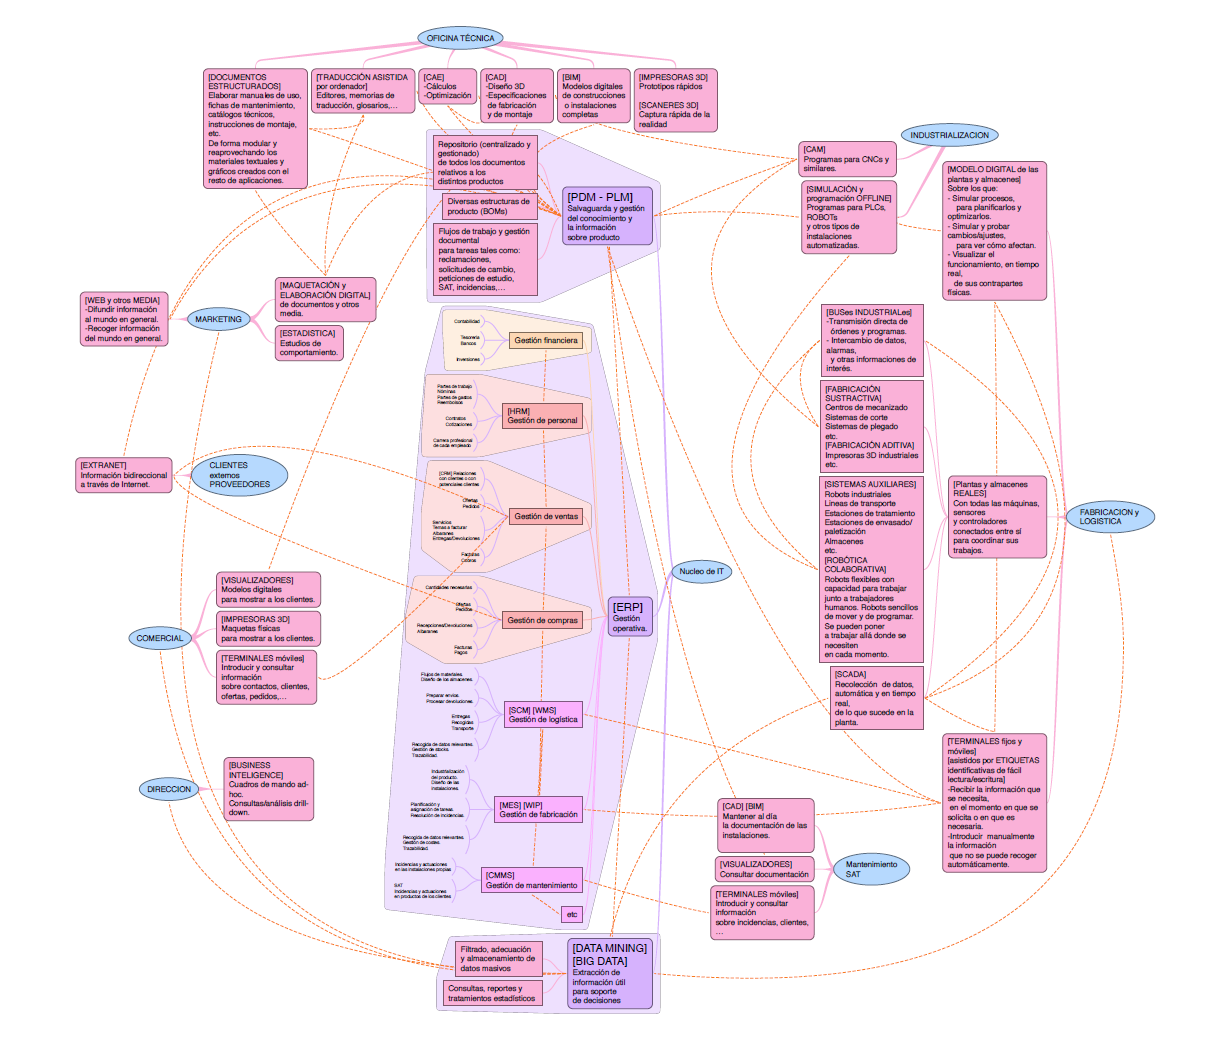
\includegraphics[width=1.1\textwidth]{Esquema general de los flujos de informacion en una empresa digitalizada}

Imagen descargable desde \url{https://www.susosise.es/documentos/Empresa_4.0_-_Esquema_general_de_los_flujos_de_informacion_en_una_empresa_digitalizada.png}

El ``bosque'', visto así, puede parecer intimidante. Pero, a medida que vayamos analizando cada una de sus partes y comprendiendo cómo encajan en la globalidad. Se ve que es un maravilloso ecosistema lleno de vida, con múltiples sinergias entre cada una de sus partes y cada uno de sus habitantes. Un ecosistema en constante evolución, donde cada habitante aprende y se va adaptando a las diversas circunstancias que se van presentando.

\subsection{Unos comentarios importantes, que se aplican a todos los apartados siguientes}
Por un lado,  indicar que la principal intención tras el mapa es suministrar un punto de partida para reflexionar. La intención de los apartados en este capítulo es la de desmenuzar el mapa general. Irnos concentrando en puntos concretos del mismo. Mientras vamos pensando en cómo se podria aplicar todo lo citado (y más) en el caso concreto de nuestra empresa.

Conviene pensar en nuestro trabajo habitual, en casos concretos. Para tratar de imaginarnos cómo se podrian desarrollar estos si tuvieramos en todo momento, al alcance de la mano, todos los datos necesarios. (Nota: La reflexión comienza por imaginarnos cuáles son o podrian ser esos ``datos necesarios''. Sin limitarnos solo a los que manejamos en la actualidad.)

Los ejemplos de operaciones que se indican aquí son meramente orientativos. Quien trabaja en cada uno de los departamentos citados pensará en muchas otras operaciones y tareas habituales en su día a día. Lo dicho, esto es un mapa general ilustrativo, no pretende ser algo exhaustivo.

Un par de puntualizaciones prácticas:
\begin{itemize}

\item Cuando se dice ``Registran...'' se quiere decir que cada dato a registrar se guarda en el sistema en el mismo momento en que se tiene conocimiento de él. 
\begin{itemize}
\item Si al registrar algo hay alguna duda, se aplica lo de ‘más vale tener datos incompletos que no tener ningún dato’. Eso sí, se ha de resolver la duda en el menor tiempo posible y completar los datos en cuanto se haya resuelto.
\item Si más tarde se descubre algún error en los datos. La misma persona que lo descubre se encarga de corregirlo. Si alguien habia utilizado el dato erróneo para algo, tendrá que ajustar también su actuación en cuanto detecte la discrepancia. 
\item Es conveniente cruzar información siempre que sea posible (por ejemplo, tener el pedido de compra a la vista siempre que se registra un albarán de recepción). Es conveniente realizar consultas de comprobación cuando se vea algo ‘raro’ o que parezca ‘no cuadrar’ con lo que se espera. 
\end{itemize}

\item Cuando se dice ``Reciben...'' o ``Consultan...'' esa consulta es, obviamente, digital. 
\begin{itemize}
\item El equipamiento informático es barato. Se presupone que hay dispositivos (pantallas) suficientes para que cualquiera que necesite procesar un dato tenga siempre a mano algún dispositivo adecuado para hacerlo.
\item La capacidad de procesamiento de esos dispositivos permite realizar con agilidad búsquedas y análisis sobre la información contenida en el sistema. Se presupone que cada persona tiene la suficiente habilidad en el manejo del sistema como para saber buscar por sí misma lo que necesita en cada momento. (nota: No solamente saber lo habitual, sino también tener suficiente conocimiento general como para resolver situaciones puntuales, o incluso extraordinarias, por sí misma.)
\end{itemize}

\end{itemize}


\subsection{Las personas encargadas de las ventas}
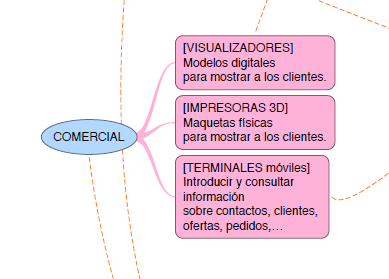
\includegraphics[width=0.65\textwidth]{subesquema - ventas01}
\\\\ 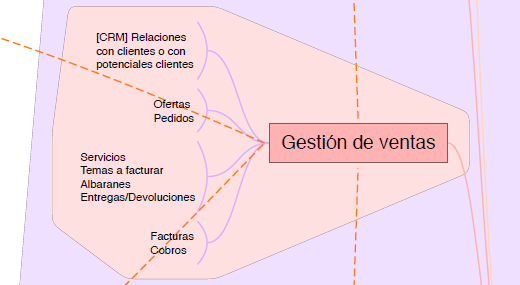
\includegraphics[width=\textwidth]{subesquema - ventas02}
\\\\ 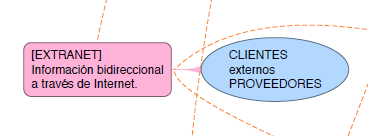
\includegraphics[width=0.65\textwidth]{subesquema - ventas03}

Registran en el ERP la interacción con los clientes (datos, ofertas, pedidos, consultas, incidencias,...). 

Registran en el ERP las listas de precios. Para ello, consultan en el ERP información sobre costes, volumen de pedidos,...

Consultan en el ERP información sobre la disponibilidad de inventarios, las previsiones de fabricación, la carga de trabajo de las personas encargadas de proveer servicios,... Para elaborar y lanzar los despachos de pedidos. 

Reciben notificación de incidencias con los pedidos a servir, incidencias en cobros,... Para gestionarlas y solventarlas.

Cada cliente puede consultar (en el ERP) el estado de sus datos, ofertas, pedidos, consultas, incidencias,... (la parte que se desee compartir con él).

Cada cliente, puede consultar (en el PDM) la información (guias de uso, guias de mantenimiento,...) que necesita para utilizar los productos que ha comprado.

\subsection{Las personas encargadas de las compras}
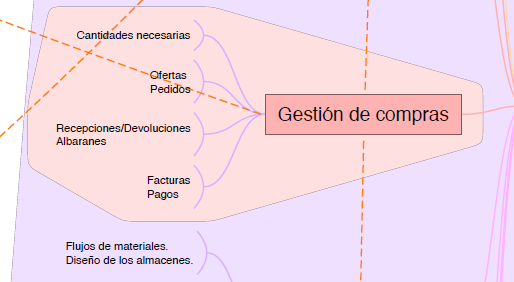
\includegraphics[width=0.9\textwidth]{subesquema - compras01}
\\\\ 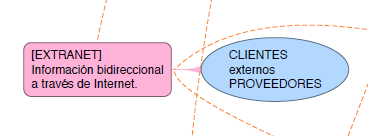
\includegraphics[width=0.65\textwidth]{subesquema - compras02}

Registran en el ERP la interacción con los proveedores (datos, ofertas, pedidos, consultas, incidencias,...). 

Consultan en el ERP información sobre la disponibilidad de inventarios, las previsiones de pedidos, las previsiones de fabricación,... Para elaborar y lanzar los pedidos que sean necesarios.

Reciben solicitudes para trasladar a los proveedores consultas sobre posibilidades, precios, disponibilidades,... Responden a los solicitantes con la información recabada.

Cada proveedor puede consultar (en el ERP) el estado de sus datos, ofertas, pedidos, consultas, incidencias,... (la parte que se desee compartir con él).

Cada proveedor subcontratado para fabricar producto, puede consultar (en el PDM) la información (diseño, especificaciones,...) que necesita para fabricarlo.

\subsection{Las personas encargadas del almacenaje\\y de las recepciones/envios de materiales}
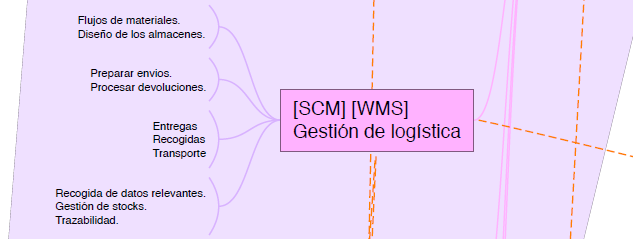
\includegraphics[width=\textwidth]{subesquema - logistica01}
\\\\ 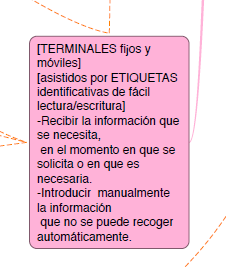
\includegraphics[width=0.4\textwidth]{subesquema - logistica02}

Reciben peticiones para servir pedidos o para mover materiales de un almacén a otro.

Registran en el ERP los envios de materiales y los acuses de recibo en destino (si procede). 

Registran en el ERP las recepciones de materiales y las ubicaciones donde quedan almacenados.

Consultan en el ERP los materiales pendientes de recibir o pendientes de enviar en cada almacén.  

Reciben notificación de incidencias con los movimientos de material, con las entregas,... Para gestionarlas y solventarlas.

\subsection{Las personas encargadas de los servicios post-venta}
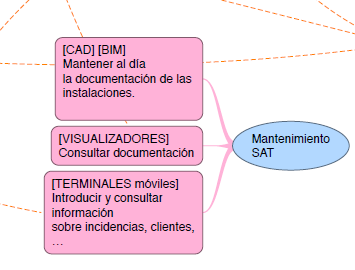
\includegraphics[width=0.5\textwidth]{subesquema - postventa01}
\\\\ 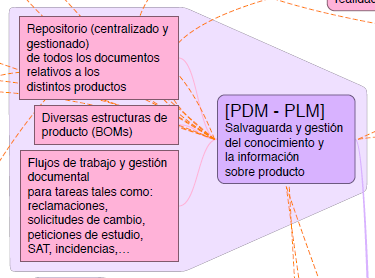
\includegraphics[width=0.7\textwidth]{subesquema - postventa02}

Reciben peticiones para atender a los clientes. Registran en el ERP los servicios realizados y las incidencias relacionadas con ellos.

En el caso de instalaciones grandes o personalizadas, elaboran y recopilan información detallada para documentar cada instalación. Registran dicha información en el PDM.

Consultan en el PDM información acerca de diseños, especificaciones, manuales de servicio,... de cada producto que han de atender.

\subsection{Las personas encargadas de la fabricación de producto}
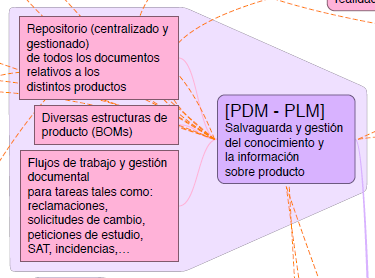
\includegraphics[width=0.6\textwidth]{subesquema - fabricacion01}
\\ 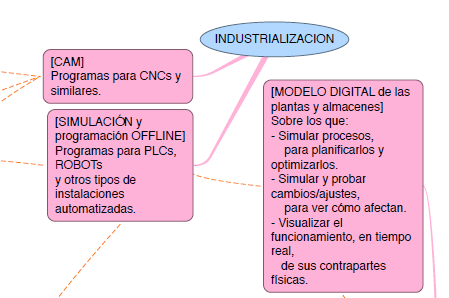
\includegraphics[width=0.7\textwidth]{subesquema - fabricacion02}
\\ 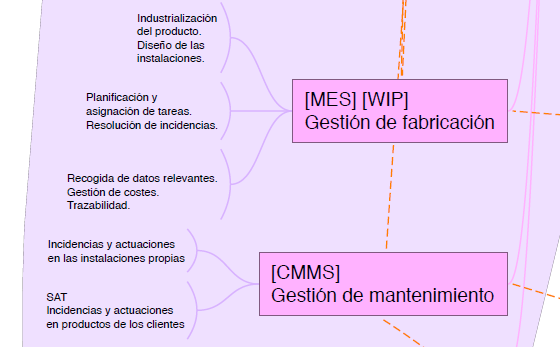
\includegraphics[width=0.9\textwidth]{subesquema - fabricacion04}
\\ 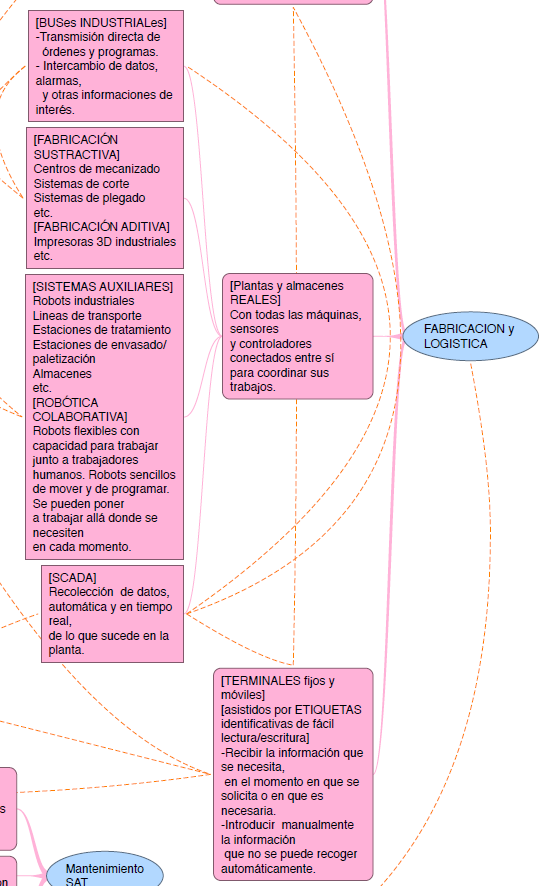
\includegraphics[width=\textwidth]{subesquema - fabricacion03}

Consultan en el ERP información sobre la disponibilidad de inventarios, las previsiones de pedidos, el estado de las compras, la disponibilidad de los recursos productivos,... Para elaborar y lanzar las órdenes de fabricación que sean necesarias.

Registran en el ERP información sobre la ejecución de las órdenes de fabricación.

Reciben notificación de incidencias en los trabajos en curso, en las instalaciones,... Para gestionarlas y solventarlas.

Consultan en el PDM información acerca de diseños, especificaciones, requisitos,... de cada producto que han de fabricar. Con los productos habituales, para guiar el proceso de fabricación. Con los productos nuevos, para elaborar y establecer los procesos de fabricación pertinentes.

Realizan simulaciones acerca de los flujos de materiales en la planta, teniendo en cuenta las capacidades reales de la misma. En el corto plazo, para estudiar el impacto de las incidencias y buscar la mejor forma de solventarlas. En el largo plazo, para mejorar y optimizar los procesos de fabricación.

\subsection{Las personas encargadas de las infraestructuras}
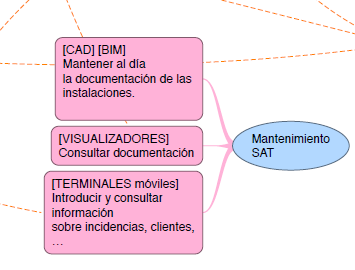
\includegraphics[width=0.55\textwidth]{subesquema - infraestructuras01}
\\ 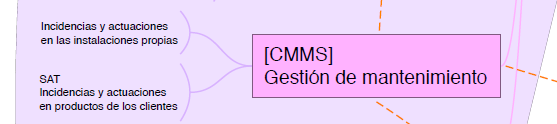
\includegraphics[width=0.9\textwidth]{subesquema - infraestructuras02}
\\\\ 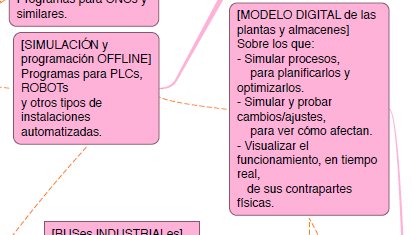
\includegraphics[width=0.6\textwidth]{subesquema - infraestructuras04}
\\ 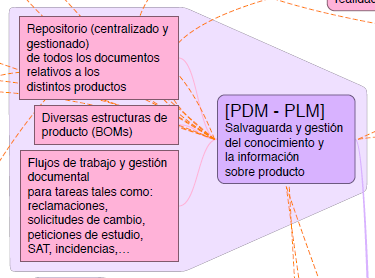
\includegraphics[width=0.5\textwidth]{subesquema - infraestructuras03}

Reciben notificación de incidencias en las instalaciones,... Para gestionarlas y solventarlas.

Consultan en el PDM información acerca de diseños, especificaciones, manuales de servicio,... de cada instalación que han de atender.

Diseñan e implementan mejoras en las instalaciones existentes y ampliaciones con nuevas instalaciones. El diseño y la programación de los nuevos sistemas se realizan sobre un gemelo digital de la planta, reduciendo así el impacto de los cambios cuando estos se han de ejecutar en la planta física real.  Elaboran y recopilan información detallada para documentar cada instalación. Registran y mantienen actualizada toda esa información en el PDM.

\subsection{Las personas encargadas del diseño de producto}
\includegraphics[width=\textwidth]{subesquema - diseño01}

Diseñan nuevos productos y estudian mejoras en los productos existentes. El diseño, los cálculos, los ensayos y las simulaciones se realizan primero sobre modelos digitales y luego sobre prototipos físicos.  Elaboran información detallada para documentar cada producto, incluyendo tanto los aspectos necesarios para su fabricación, como para su servicio, como para su utilización. 

Registran y mantienen actualizada toda esa información en el PDM.

Reciben notificación de peticiones de cambios, incidencias,... Para gestionarlas y solventarlas.

\subsection{Las personas encargadas de la promoción de los productos y servicios que ofrece la empresa}
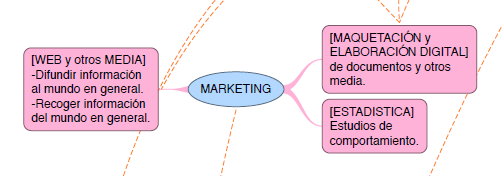
\includegraphics[width=0.9\textwidth]{subesquema - marketing01}

Consultan en el PDM información acerca de diseños, especificaciones, manuales de servicio, manuales de uso,... de los productos.

Elaboran documentación y materiales multimedia de promoción. 

Elaboran y supervisan la imagen corporativa en todos los documentos que se utilicen fuera de la empresa. Registran y mantienen actualizada toda esa información en el PDM.

Reciben notificación de las incidencias y quejas de los clientes,... Para gestionarlas y solventarlas.

Consultan en el repositorio de datos (DATA MINING, BIG DATA), para elaborar y destilar la información que necesitan para diseñar campañas de publicidad y para tomar decisiones acerca del desarrollo de producto.

(nota: IT se encarga de la captura, filtrado, adecuación y almacenamiento de los datos en bruto. Para que estén disponibles en un formato adecuado para la consulta y elaboración de información por parte de los usuarios, que utilizarán para ello las herramientas de mineria de datos correspondientes.)

\subsection{Las personas encargadas de los cobros y los pagos}

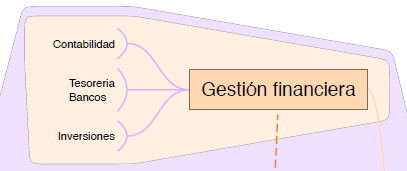
\includegraphics[width=0.6\textwidth]{subesquema - finanzas02}

Registran en el ERP las previsiones de necesidades financieras y los movimientos reales de dinero (cobros, pagos, inversiones,...). 

Reciben notificación de incidencias con los pagos, con los cobros,... Para gestionarlas y solventarlas.

Registran en el ERP los preceptivos registros contables y elaboran las cuentas legales.

\subsection{Las personas encargadas de las personas}
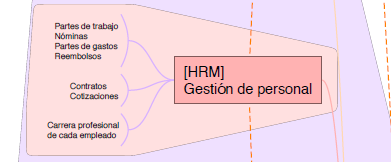
\includegraphics[width=0.7\textwidth]{subesquema - personal01}

Consultan en el ERP los partes de trabajo, partes de gastos,... Para elaborar y liquidar las nóminas y otros pagos.

Reciben notificación de incidencias con las nóminas, las cotizaciones,... Para gestionarlas y solventarlas.

Registran en el ERP los datos relativos a cada empleado.

\subsection{Las personas encargadas de dirigir la empresa}
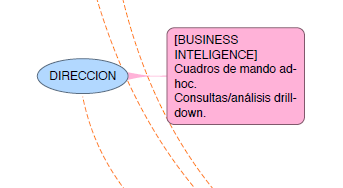
\includegraphics[width=0.6\textwidth]{subesquema - direccion01}

Consultan en el ERP la información relativa a la marcha de la empresa.

Reciben notificación de incidencias graves,... Para gestionarlas y solventarlas.

Consultan en el repositorio de datos (DATA MINING, BIG DATA), para elaborar y destilar la información que necesitan para tomar decisiones.

(nota: IT se encarga de la captura, filtrado, adecuación y almacenamiento de los datos en bruto. Para que estén disponibles en un formato adecuado para la consulta y elaboración de información por parte de los usuarios, que utilizarán para ello las herramientas de mineria de datos correspondientes.)



\newpage
\section{Resumen de las tecnologias involucradas}

\subsection{Las personas}
Para aprovechar plenamente las nuevas capacidades tecnológicas de los sistemas, son necesarios cambios en la forma de utilizarlos. 

Para ello, es imprescindible ajustar en concordancia la capacidad de las personas que manejan esos sistemas. 

Esta es la parte más costosa de la adaptación, ya que a los humanos nos suele costar bastante desaprender formas de trabajar ya conocidas para aprender nuevas formas de trabajar.

Pero es la parte más importante. Y a la que se debe dedicar más recursos.

\subsection{El ERP}
Núcleo central de toda la información operativa de la empresa. Entendiendo por información operativa la relativa a todos los aspectos del día a día de la misma. 

No solo en el ámbito financiero (intercambio de dinero), sino también en el físico (intercambio de materiales) y en el abstracto (intercambio de servicios).

Ver más detalles en la sección \ref{ERP}, página \pageref{ERP}.


\subsection{El PDM-PLM}
Núcleo central de toda la información relativa a producto/servicio/instalaciones. Desde los modelos de fabricación hasta los manuales de servicio, pasando por cualquier documento que apoye/informe cualquier proceso.


Ver más detalles en la sección \ref{PDM}, página \pageref{PDM}.


\subsection{El repositorio ``BigData''}
Núcleo central que guarda (casi)todos los datos presentes, pasados y futuros que pudieran tener alguna relevancia. Junto con las adecuadas herramientas para filtrarlos y tratarlos, es un apoyo imprescindible para el análisis de situaciones y la toma de decisiones.

Ver más detalles en la sección \ref{DATA}, página \pageref{DATA}.


\subsection{Las redes de comunicaciones}
La columna vertebral de todo el sistema. Sin la capacidad de transportar datos de forma fiable y segura hasta donde se vayan a utilizar, poca utilidad tendrán esos datos.

Ver más detalles en la sección \ref{redes_de_comunicaciones}, página \pageref{redes_de_comunicaciones}.

\subsection{Otras tecnologias}

\subsubsection*{Visualización}
La información se puede compartir o analizar de forma más eficiente con el apoyo de sistemas gráficos que la muestren allá donde se necesite, en un formato fácil de entender y con capacidad para interactuar con ella en tiempo real.

Un paso en ese sentido son las nuevas pantallas tactiles, de todos los tamaños y formatos, con más o menos capacidad de proceso local: móviles, tablets, pizarras digitales,...

\subsubsection*{Datos ubicuos (la ``nube'')}
La información es más eficaz si es posible trabajar con ella en cualquier lugar donde nos encontremos y con cualquier dispositivo que tengamos a mano en ese momento.

La forma de conseguir eso es contar con la ubicuidad de Internet. Bien de la manera más sencilla, contratando el servicio a un proveedor ``on-line'' (los datos residen en los servidores del proveedor). O bien de la más compleja, estableciendo nuestro propio servicio ``on-premise'' (los datos residen en nuestros servidores locales).

\subsubsection*{Seguridad}
Cuanto más interconectados estamos, más importante es dotarnos de los adecuados mecanismos de seguridad para evitar/detectar accesos no autorizados.

Es importante tener en cuenta que no existe la seguridad ``absoluta''. Al igual que no existe la seguridad ``automática/transparente''. La seguridad es siempre un ``toma y daca'' entre quienes se quieren proteger y quienes quieren atacar los recursos protegidos; sin perder de vista las personas que simplemente ``se ven afectadas'' por unos u otros en cada momento.

En el diseño de todo sistema de seguridad es necesario analizar y ponderar adecuadamente los activos a proteger, el valor que puedan tener para un potencial atacante, los riesgos que les puedan afectar y las pérdidas que se puedan sufrir en caso de problemas con ellos.

Lo más importante al diseñarlo: conseguir un adecuado equilibrio entre el grado seguridad necesario y el grado de afectación tolerado por los usuarios en su trabajo.

Las circunstancias cambian. Un sistema de seguridad eficaz requiere de un mantenimiento continuado y de revisiones periódicas para mantenerlo actualizado.

\subsubsection*{Gemelos digitales (``digital-twin'')}
Hoy en día, prácticamente cualquier sistema, proceso o producto es susceptible de ser simulado digitalmente con la precisión necesaria como para que se pueda ``trabajar'' sobre él tal y como se haria sobre el sistema, proceso o producto real.

Ni que decir tiene que resulta mucho más barato y flexible trabajar con un modelo virtual que con un sistema físico. Esto permite explorar más alternativas y realizar estudios más detallados sobre cualquier actuación que se pretenda realizar, antes de realizarla.

\subsubsection*{Automatización avanzada}
Con el apoyo de sensórica avanzada (por ejemplo, visión artificial), de sistemas capaces de procesar gran cantidad de sensores y de sistemas capaces de ``entender'' toda esa información (inteligencia artificial). Las máquinas se van encargando de cada vez más y más procesos antes reservados para humanos. 

\subsubsection*{Fabricación avanzada}
Incluyendo, pero no limitándose, a las nuevas técnicas de fabricación aditiva que complementan las tradicionales técnicas de fabricación substractiva.

Por fabricación avanzada se entiende el proceso de pasar del diseño o pedido al producto terminado entregado al cliente; con la flexibilidad necesaria para acomodar la ``personalización en masa'' (fabricación ad-hoc, según la demanden las circunstancias)

Algunos ejemplos:
\begin{itemize}
\item Interconexión directa entre máquinas, para que puedan coordinar sus trabajos.
\item Interconexión directa entre el sistema de gestión de producción, los puestos de trabajo y las máquinas. Para coordinar todo el proceso.
\item Robótica colaborativa, suficientemente flexible como para irla adaptando en cada momento a las tareas donde sea útil su apoyo en ese momento.
\item etc.
\end{itemize}

\vspace{1cm}
Mas información sobre estos aspectos en el siguiente capítulo\ldots


\chapter{En qué afecta la transformación digital al producto.}

Las nuevas tecnologias digitales nos permiten:
\begin{itemize}
\item Diseñar con más detalle/realismo, en 3D y con información adicional (comportamiento físico, planificación temporal, sistemas de control,\ldots). Creando modelos digitales que contengan dentro de ellos los aspectos más importantes de los objetos reales que estamos diseñando.
\item Ensayar esos diseños con programas de cálculo y simulación. Completando el diseño según vemos ``trabajar/comportarse'' al modelo de forma virtual, en la pantalla de un ordenador.
\item Instrumentar la realidad construida a partir de esos diseños. Para captar datos y realimentar con ellos los modelos virtuales y las simulaciones de los pasos anteriores. De tal forma que se puedan ir mejorando.
\end{itemize}


\section{Fase de diseño y concepción}\label{diseño_de_producto}
CAD (Computer Aided Design)
\\CAE (Computer Aided Engineering)
\\AR (Augmented Reality) - VR (Virtual Reality)

El producto se puede diseñar, calcular, probar y optimizar (casi) por completo en un entorno virtual:

\begin{itemize}
\item Software CAD permite preparar un \textbf{modelo digital del producto}. Recogiendo todos los aspectos que lo definen:
\begin{itemize}
\item su forma [geometria 3D],  
\item sus requisitos de fabricación (cotas, restricciones dimensionales, tratamientos superficiales,\ldots) [anotaciones PMI], 
\item sus propiedades características (materiales, códigos, especificaciones,\ldots), 
\item etc.
\end{itemize}

Es decir, el modelo digital contendrá toda la información que define de forma completa el producto.

En las fases iniciales de diseño puede resultar de utilidad usar algún software de \textit{diseño generativo}. Estos softwares permiten generar, calcular, analizar y filtrar automáticamente multitud de posibilidades ajustadas a las restricciones de diseño que se impongan. De esta forma se pueden explorar y valorar muchas más  alternativas de diseño de las que seria posible valorar de forma manual.

\item Software CAE permite \textbf{simular, calcular y analizar el comportamiento físico} del producto en diversos aspectos: mecánico, electromagnético, térmico,\ldots
\\Tanto para verificar su adecuación a los requisitos y estándares legales que le fueran de aplicación. Como para optimizarlo en diversos aspectos que puedan interesar.

\item Software de animación y renderizado, complementado en su caso con dispositivos AR o VR, permite visualizar y analizar el \textbf{comportamiento funcional} del producto.
\end{itemize}

Si todo este proceso virtual de definición del producto se quedara corto en algún punto, seria el momento de recurrir a los tradicionales prototipos físicos.

\subsection*{Algunas referencias ilustrativas}
\url{https://www.onshape.com/en/}
\\ \url{https://www.autodesk.com/products/fusion-360/overview}
\\ \url{https://www.plm.automation.siemens.com/global/es/products/nx/}
\\ \url{https://graphisoft.com/es/solutions/products/archicad}
\\ \url{https://www.solidworks.com/es/solutions}

::: Modelo digital del producto :::
\\ \url{https://develop3d.com/product-design/pmi-3d-annotation-the-drawing-killer/}
\\ \url{https://www.appliedcax.com/resources/advanced-manufacturing-product-manufacturing-information-and-model-based-definition}
\\ \url{https://avantek.es/productos/software-de-mecatronica-industrial-de-siemens/}
\\ Integración diseño eléctico y mecánico: \url{https://youtu.be/fB58ZHMrrJs} \url{https://youtu.be/8NYWx9f0l5Q}
\\ El edificio virtual. BIM con Archicad: \url{https://youtu.be/HHBGAKsB2b4}

::: Diseño generativo :::
\\ \url{https://www.autodesk.com/solutions/generative-design}
\\ \url{https://solidedge.siemens.com/en/solutions/products/3d-design/next-generation-design/generative-design/}
\\Demo en Solid Edge ST10: \url{https://youtu.be/7zPnaDLKSPM?t=534}
\\ \url{https://www.ptc.com/es/technologies/cad/generative-design}
\\ \url{https://towardsdatascience.com/ai-architecture-and-generative-design-e22320828d46}

::: CAE :::
\\ \url{https://www.plm.automation.siemens.com/global/en/products/simcenter/femap.html}
\\ \url{https://iberisa.wordpress.com/category/tutoriales/}
\\ \url{https://maplesoft.com/products/maplesim/}
\\ \url{https://www.maplesoft.com/solutions/engineering/AppAreas/Virtual-Commissioning.aspx}
\\ \url{https://es.mathworks.com/products/simulink.html}
\\ {\footnotesize \url{https://www.plm.automation.siemens.com/global/en/products/simulation-test/system-simulation.html}}
\\ \url{https://www.scia.net/en/software/scia-engineer}
\\ \url{https://www.comsol.com/}
\\ \url{https://www.cm-labs.com/vortex-studio/}
\\ \url{https://www.beta-cae.com/ansa.htm}
\\ \url{http://www.lstc.com/products/ls-dyna}
\\ \url{https://www.mscsoftware.com/product/msc-nastran}
\\ \url{https://www.mscsoftware.com/product/adams}
\\ \url{https://www.ansys.com/products/fluids/ansys-fluent}
\\ \url{https://www.ansys.com/products}
\\ \url{https://www.openfoam.com/}
\\ \url{https://www.mentor.com/products/}
\\ \url{https://www.gompute.com/hpc-cloud/}
\\ \url{https://www.altair.com/mechatronics/}
\\ \url{https://www.altair.com/digital-twin/}
\\ \url{https://www.solidworks.com/product/3dexperience-works-simulation}

::: AR/VR :::
\\ \url{https://varjo.com/solutions/}
\\ \url{https://www.cm-labs.com/vortex-studio/solutions/human-in-the-loop/}
\\ \url{https://varjo.com/case-kia-autodesk-vred-driving-the-future-with-xr-collaboration-in-car-design/}

\section{Fase de construccion/fabricación}\label{fabricacion_de_producto}
CAM (Computer Aided Manufacturing)
\\VDC (Virtual Design and Construction)
\\DfMA (Design for Manufacturing and Assembly)
\\AWP (Advanced Work Packaging)

Como se comenta en capítulos posteriores, (\ref{fabricacion_digital} y \ref{simulacion_de_procesos} en la página \pageref{fabricacion_digital}), la fabricación/construcción del producto se puede preparar y optimizar de forma virtual, antes de ejecutarse en la realidad.

El modelo digital citado en la sección anterior, sirve de referencia durante todas las operaciones de fabricación y los trabajos de construcción; tanto virtuales como reales.

Además, en productos complejos (como por ejemplo: plantas industriales, buques, edificios,\ldots), el modelo digital sirve también como registro de lo realmente fabricado/construido (modelo ``as-build''). Recogiendo las modificaciones que van surgiendo con respecto a lo inicialmente diseñado.

Disponer de un modelo completo de producto facilita la división del mismo en distintos módulos y facilita la planificación de su fabricación en distintos paquetes de tareas. Esto permite repartir tareas y pre-fabricar módulos en distintas ubicaciones especializadas, para luego ensamblarlos en el producto final.

Esta tendencia hacia la prefabricación modular se está potenciando en cada vez más ámbitos, gracias a que:
\begin{itemize}
\item El diseño y la planificación digital permiten coordinar con precisión las distintas partes que luego han de unirse en el producto final.
\item Las comunicaciones digitales permiten coordinar con agilidad dudas o imprevistos que puedan surgir entre los diversos equipos participantes. 
\item Los medios de captura y digitalización de la realidad permiten controlar el avance real de los trabajos parciales y reaccionar así con efectividad ante las desviaciones que se van produciendo.
\end{itemize}

{\footnotesize \url{https://www.plm.automation.siemens.com/global/es/products/manufacturing-planning/manufacturing-work-instructions.html}}
\\{\small \url{https://www.plm.automation.siemens.com/global/es/products/nx/nx-for-manufacturing.html}}

\url{https://www.marine.sener/es/foran}

\url{https://www.e-builder.net/product/project-lifecycle/#Procurement}
\\ \url{https://www.bentley.com/es/products/product-line/construction-software/synchro-4d}
\\A Smarter Way to Build: \url{https://www.youtube.com/watch?v=j6PqIidY8ts}
\\ Prefabricated 9 level building goes up in 5 days:
\\ \url{https://www.youtube.com/watch?v=CYZXNDKoGtA&t=15}
\\Offsite Management School: \url{https://www.youtube.com/watch?v=8pqmg18p2pA}
\\MiC - Modular Integrated Construction: \url{https://www.youtube.com/watch?v=t-cj-kAJbvY}

\section{Fase de utilización}
FM (Facilty Management)
\\IoT (Internet of Thigs)
\\sensórica avanzada

Los productos complejos (como por ejemplo: plantas industriales, buques, edificios,\ldots), después de fabricados y entregados al cliente, requieren manejar mucha información para su correcta operación y mantenimiento. Esta fase de su vida también puede beneficiarse de algunas las tecnologias comentadas en las fases anteriores.

En concreto, el modelo digital con toda la información del producto, convenientemente actualizado a lo realmente construido, es de inestimable ayuda en esta fase. Y para que siga siendo de ayuda, ha de mantenerse actualizando según se van realizando cambios en las intervenciones de mantenimiento.

Redes de sensores repartidos por todo el producto. Ayudan a monitorizarlo y a explotarlo de manera eficiente en su funcionamiento del día a día. Detectando de forma precoz problemas que requieran una intervención de mantenimiento.

Tecnologias de telepresencia permiten realizar intervenciones remotas o consultas con personas expertas. Sin necesidad de desplazamientos  físicos por parte de estas a donde esté ubicado el producto.

\url{https://www.e-builder.net/product/project-lifecycle/#Operations}
\\ \url{https://www.ibm.com/es-es/products/maximo/industries}
\\ \url{https://www.ultramain.com/}


\section{Fase de retirada}

El modelo digital con información del producto, convenientemente actualizado a los cambios que hayan podido surgir durante toda su vida, es de inestimable ayuda en esta fase. Ya que permite un mejor desmantelamiento y reciclaje. 


\chapter{En qué afecta la transformación digital a la fabricación de producto.}

En la fabricación de producto, las tecnologías digitales permiten un mayor conocimiento (y, por ende, mayor optimización) tanto del propio producto como de los procesos de fabricación que permiten hacerlo realidad.

Además, las tecnologías de automatización de procesos y sistemas productivos permiten fabricar de forma personalizada con una eficiencia parecida\footnote{Realmente el coste por unidad producida siempre será algo mayor en la fabricación personalizada que en la fabricación en masa. Pero su ventaja reside en que permite lanzar series más cortas y mejor adaptadas a la demanda de cada momento.} a la obtenida con la fabricación en masa. 



\vspace{0.5cm}

\url{https://www.aiscorp.com/factory-4-0/industry-4-0/}
\\ \url{https://www.aiscorp.com/factory-4-0/digital-thread/}

¿Qué es realmente un gemelo digital? tipos, diferencias y casos de uso
\\ \url{https://youtu.be/W0nmq0fwyYU}



\section{Gestión y monitorización de la planta}
SCADA (Supervisory Control and Data Adquisition)
\\DCS (Distributed Control Systems)
\\IoT (Internet of Things)

\textbf{Etiquetas identificadoras} colocadas sobre ciertos elementos, junto con los correspondientes lectores colocados allá donde sea necesario, permiten realizar un seguimiento automatizado de esos elementos a lo largo de todo el proceso.

\textbf{Terminales por doquier} permiten a cualquier operario consultar información (órdenes, diseños, instrucciones, procedimientos,\ldots) de lo que se está produciendo y de las operaciones a realizar. 

Esos mismos terminales permiten también que cualquier persona registre, sobre la marcha, lo que va sucediendo. Complementando con ello los datos recogidos directamente desde las máquinas y dispositivos de producción.

\textbf{Dispositivos de escaneo y medición} digitales (palpación, laser, lidar, fotogrametria, visión industrial,\ldots) integrados en algunos terminales permiten realizar comprobaciones de calidad (semi)automatizadas. 

\textbf{Redes industriales} interconectando todos los CNCs, PLCs, terminales, sensores,\ldots permiten un trafico fluido y seguro de información entre todos ellos.
\\\textbf{Dispositivos y sensores IoT}, habitualmente inalámbricos, permiten monitorizar y captar datos en prácticamente cualquier ubicación, incluso en movilidad.
\\ Sistemas de registro y \textbf{monitorización} de comunicaciones permiten mantener el tráfico fluido y seguro.

Entornos \textbf{SCADA} habilitan la recolección, procesamiento y visualización de todos los datos para convertirlos en información útil. Permitiendo evaluar y conocer en tiempo real lo que está sucediendo en la planta (monitorización continua).
\\Además, el análisis de datos históricos permite detectar tendencias y puntos de posible mejora.

Entornos \textbf{DCS} permiten manejar la planta de forma centralizada desde centros de control centralizados, valga la redundancia.

\subsection*{Algunas referencias ilustrativas}
Ejemplo real de una planta digitalizada:
\\ \url{https://www.youtube.com/watch?v=Q4BK4qy0Ts4&t=67s}
\\Ejemplo de una planta de demostración: 
\\ \url{https://www.youtube.com/watch?v=kbNwSJyZz1w}
\\ \url{https://www.mmsonline.com/articles/getting-started-with-machine-monitoring}
\\ \url{https://new.siemens.com/global/en/products/automation/systems/cnc-sinumerik/digitalization/manufacturing.html}
\\ Central Data Management: 
\\ \url{https://www.youtube.com/watch?v=JCYx7ImVPKw}
\\Interactive Communication platform - ActiveCockpit:
\\ \url{https://www.youtube.com/watch?v=PPdxGQQZF6U}
\\ Paperless Machine Shop:
\\ \url{https://vimeo.com/506147681} Going Paperless with ProShop
\\ \url{https://vimeo.com/364150066} ProShop Short Overview
\\ \url{https://www.proshoperp.com/company/video-library/}
\\ \url{https://www.proshoperp.com/company/video-library/#Modules}

::: redes de comunicacion :::
\\Ver la sección \ref{redes_de_comunicaciones}, en la página \pageref{redes_de_comunicaciones}.

::: DWI (Digital Work Instructions) :::
\\ \url{https://www.aiscorp.com/solutions/digital-manufacturing-engineering/}
\\ {\footnotesize \url{https://www.plm.automation.siemens.com/global/es/products/manufacturing-planning/manufacturing-work-instructions.html}}
\\ módulo `Publicaciones Técnicas' de Solid Edge:
\\ \url{https://www.youtube.com/watch?v=cLK9z97ep0s&t=70}
\\ módulo NX CAM Work Instruction Authoring: 
\\ \url{https://youtu.be/jPA9HmZ938E}

:::
\\ Sistema de información para máquinas forestales:
\\ \url{https://www.ponsse.com/es/productos/sistemas-de-informacion#/}
\\ Realidad aumentada para asistencia técnica remota:
\\ \url{https://www.kognitivspark.com/}


\section{Diseño, simulación, programación y optimización de máquinas e instalaciones productivas}\label{fabricacion_digital}
TIA (Totally Integrated Automation)
\\``Virtual Commisioning'' (puesta en marcha virtual) 

Los actuales entornos de simulación permiten elaborar modelos virtuales que son prácticamente ``duplicados digitales'' (gemelo-digital, digital-twin) de las máquinas e instalaciones reales. 

Estos simuladores permiten programar los equipos y ajustar (casi)completamente su operación dentro del entorno virtual (preparación off-line), minimizando así las paradas de preparación en los equipos físicos reales.

\begin{itemize}
\item Para las máquinas de control numérico CNC. Se parte de la definición digital de la pieza (\begin{footnotesize}ver \ref{diseño_de_producto}, página \pageref{diseño_de_producto}, `modelo digital del producto'\end{footnotesize}), y se definen las operaciones de mecanizado/corte/adicción/\ldots necesarias para fabricarla. Los modernos programas CAM ofrecen recursos para simular y optimizar esas operaciones en un entorno virtual fuera de la máquina. Este entorno virtual puede ser:
\begin{itemize}
\item Simulador genérico, según tipo de herramienta (torno, fresa,\ldots). Tiene la pega de requerir luego un postprocesador específico para convertir el programa CNC creado por el CAM a uno específico para la máquina y perifericos concretos donde se vaya a cargar.
\item Simulador específico para la máquina y periféricos concretos que se vayan a utilizar, con el postprocesador integrado. Capaz de simular teniendo en cuenta las capacidades y limitaciones reales del equipamiento. Tiene la ventaja de que el programa CNC se optimiza para sacar el máximo partido posible del equipo disponible.
\end{itemize}

\item Para los robots, cintas transportadoras y otros dispositivos controlados por PLCs o similares.
\begin{itemize}
\item Se obtiene (normalmente del propio fabricante) modelos en 3D de su forma externa y de las articulaciones entre sus distintas partes.
\item Sobre esos modelos, se puede simular su movimiento; para planificarlo, coordinarlo y optimizarlo. 
\item Esta simulación es físicamente realista y se realiza en conexión con PLCs y controladores concretos (reales o virtualizados).
\end{itemize}
De esta forma se va ajustando el replanteo de la instalación y se van preparando offline los correspondientes programas a cargar en sus dispositivos. 

\item Para equipos auxiliares diseñados ad-hoc. En su diseño se aplican las técnicas comentadas en el apartado \ref{diseño_de_producto}, página \pageref{diseño_de_producto}. Generando para ellos modelos virtuales sobre los que simular su operación, tal y como se ha comentado en los puntos anteriores.
\end{itemize}

Es importante disponer de un sistema centralizado de almacenamiento para guardar en él todos los programas de control generados. Normalmente, ese almacenamiento suele estar ligado al sistema PDM que alberga los datos de producto. Este  repositorio de programas se complementa con un sistema de comunicaciones entre repositorio y todos los CNC, PLCs y demás controladores en planta. De esta forma se pueden telecargar los programas adecuados según se requiera para fabricar tal o cual producto en tal o cual máquina concreta.


\subsection*{Algunas referencias ilustrativas}
\url{https://new.siemens.com/mx/es/productos/automatizacion.html}
\\ \url{https://new.siemens.com/global/en/products/automation/systems/cnc-sinumerik/digitalization/manufacturing.html}
\\ Una planta digitalizada:
\\ \url{https://www.youtube.com/watch?v=Q4BK4qy0Ts4&t=67s}
\\ Una empresa con digitalización integral:
\\ \url{https://www.youtube.com/watch?v=rsMEMNh9ejw&t=64s}
\\ Una empresa con gestión centralizada de programas CNC:
\\ \url{https://www.youtube.com/watch?v=JCYx7ImVPKw}
\\ Programación offline, AGV Simulation:
\\ \url{https://youtu.be/0m7488hThGY}

::: Máquina Herramienta ::: Instalaciones Productivas :::
\\ {\small \url{https://www.plm.automation.siemens.com/global/es/products/mechanical-design/mechatronic-concept-design.html}}
\\ NX MCD (Mechatronics Concept Designer): \url{https://www.youtube.com/watch?v=PPVknHdp-2s}
\\ \url{https://www.plm.automation.siemens.com/global/en/products/manufacturing-operations-center/}
\\ \url{https://es.dmgmori.com/productos/socios-tecnologicos/siemens}
\\ \url{https://www.plm.automation.siemens.com/global/es/products/nx/nx-for-manufacturing.html}
\\ \url{http://www.volumill.com/}
\\Fusion 360 Machine Simulation: \url{https://youtu.be/JFPHMw78V94} \\\url{https://youtu.be/D2kyR4y7iNg}

::: Entornos virtuales de simulación :::
\\ \url{https://www.plm.automation.siemens.com/global/es/products/tecnomatix/}
\\ \url{https://www.emerson.com/en-us/automation/operations-business-management/dynamic-simulation}
\\ \url{https://www.cgtech.com/solutions/machine-tool-showrooms.html}
\\ \url{https://www.3ds.com/products-services/delmia/products/3dexperience/}

::: Virtual Commisioning :::
\\ Una imagen visual rápida: \url{https://youtu.be/vs3-3i9JwDI?t=106}
\\ Una explicación rápida de en qué consiste: \url{https://youtu.be/ZvrE2IfrfgI}
\\ Un pequeño ejemplo de VC, paso a paso: \url{https://www.youtube.com/watch?v=APSWlK_xL9g}
\\ Virtual Commissioning for Tecnomatix Plant Simulation and PLCSIM Advanced:
\\ \url{https://youtu.be/NMaecAEuSak?t=90}
\\ Virtual commissioning with Tecnomatix Process Simulate:
\\ \url{https://youtu.be/IoDNGvv2fDs?t=153}
\\ \url{https://www.maplesoft.com/solutions/engineering/AppAreas/Virtual-Commissioning.aspx}

\section{Diseño, simulación y optimización de procesos.}\label{simulacion_de_procesos}
``Digital Twin'' (gemelo digital) 

Entornos de simulación virtual permiten elaborar modelos digitales realistas de procesos tales como los de acopio, almacenamiento, fabricación o distribución de producto. Estos modelos (gemelo-digital, digital-twin) permiten reproducir y visualizar con fidelidad las operaciones a realizar. Siendo de inestimable ayuda a la hora de analizar y optimizar el proceso. 

No solo se modelan las instalaciones involucradas, cada máquina/equipo con sus caracteristicas reales. Sino que también se incorporan los procesos manuales, con una estimativa de rendimiento. E incluso se tienen en cuenta sucesos aleatórios, tales como averias u otros problemas, con su respectiva estimación estadística. Todo ello con la idea de conseguir un modelo lo más realista posible del proceso que se pretende estudiar.

Horas o días de trabajo en la realidad se simulan en minutos. Visualizándose los distintos flujos de materiales u otros indicadores de interés como si estuvieran sucediendo en la realidad, a la velocidad acelerada que se decida. Todo el desarrollo del proceso se guarda, para luego ser analizado en detalle o comparado con otras rondas de simulación. 

Es sencillo hacer modificaciones y probar diversos escenarios de ``qué pasaria si\ldots''. Se pueden realizar tantos ensayos como sean necesarios para llegar a familiarizarse con el funcionamiento del proceso, identificar sus puntos críticos y llegar a la mejor optimización posible.

El modelo de simulación puede servir también para monitorizar el proceso real. Tan solo hemos de utilizar sensores y otros captadores de información en los adecuados puntos de la ubicación física donde se desarrolla el proceso en la realidad. (Suelen resultar unas pantallas muy vistosas, donde es sencillo seguir la pista a lo que está sucediendo.)

En cualquier momento se pueden duplicar los datos digitales reales para iniciar una nueva simulación virtual a partir del punto real que se desee. Esta técnica es muy útil cuando suceden imprevistos a los que hay que dar la mejor solución posible. (Las pruebas de ``qué pasaria si\ldots'' siempre son más baratas y seguras de ensayar en un entorno virtual que hacerlas directamente sobre el entorno real. Y más cuando se hacen con prisas para reaccionar ante un imprevisto.)

Para cerrar el círculo, los datos históricos recogidos durante la monitorización real ayudan a refinar y mejorar el modelo de simulación. Acercándolo cada vez más a la realidad que pretende modelar.


\subsection*{Algunas referencias ilustrativas}
Simulación de una planta de alimentos: \url{https://youtu.be/lq9SU2VVHdI?t=745}
\\Analisis de datos sobre una simulación: \url{https://youtu.be/MSPD70ituCs?t=285}
\\Introduction to Plant Simulation: \url{https://youtu.be/VAVVWg5D-lM}
\\ \url{https://www.plm.automation.siemens.com/global/es/products/tecnomatix/}
\\ \url{https://www.flexsim.com/es/flexsim/}
\\ \url{https://www.lanner.com/en-gb/technology/witness-simulation-software.html}
\\ \url{https://www.nvidia.com/en-us/omniverse/solutions/digital-twins/}


\section{Fabricación flexible}
En los últimos años, todas las tecnologías antes citadas, y algunas más, vienen complementándose para permitir fabricar  series cortas (o incluso piezas individuales) de forma competitiva. 

En lugar de líneas de producción estáticas, optimizadas para un solo tipo de producto. Se pueden utilizar lineas flexibles, multipropósito, fáciles de re-configurar. Compuestas por elementos de producción modularizados y reconfigurables, fáciles de desplazar de una tarea a otra según sea necesario en cada momento. 

Los costes unitarios por elemento fabricado en estas líneas flexibles suelen ser mayores que los obtenidos con las tradicionales líneas estáticas de producción en masa.

Pero, salvo en los casos en que la demanda de grandes series sea algo inherente al propio producto, merece la pena tener en cuenta la ventaja de fabricar adaptándose a la demanda real de cada producto en cada momento.

A efectos de dar una pincelada rápida, se podrian destacar las siguientes tecnologías como claves para implementar una fábrica flexible:

\begin{description}
\item[Modelo digital del producto]: Detallando en él todo lo necesario para fabricar una determinada pieza o producto; tanto a nivel geométrico (3D) como a nivel de especificaciones (materiales, anotaciones PMI --Product Manufacturing Information-- , propiedades, comentarios,\ldots), tal y como se describe en el capítulo \ref{diseño_de_producto}, página \pageref{diseño_de_producto}.
\\Este modelo sirve como base, 
\begin{itemize}
\item para preparar la fabricación, 
\item para programar las máquinas CNC y los robots,
\item para elaborar las instrucciones a los operarios (DWI, Digital Work Instructions
\item \ldots
\end{itemize}

\item[Máquinas colaborativas entre ellas]: La conexión entre máquinas permite que funcionen como un todo continuo, notificandose unas a otras lo que necesiten para coordinar sus operaciones.
\\La sensórica avanzada permite que las máquinas reconozcan su entorno y se adapten automáticamente a él (por ejemplo, saber localizar y situar automáticamente diferentes objetos en un entorno más o menos holgado).
\\Esto posibilita una (re)programación de tareas más sencilla y rápida. 

\item[Máquinas colaborativas con humanos] (cobots): La sensórica avanzada permite que las máquinas reconozcan la presencia de humanos en su entorno y se adapten con seguridad a ellos.
\\Permite también la programación de tareas de forma visual o táctil, dando indicaciones generales y posicionamientos aproximados, sin necesidad de complicados lenguajes de programación ni de una precisión rigurosa. 
\\Posibilitando así que los propios operarios puedan adaptar el cobot a lo que se necesite en cada momento.

\item[Maquinas conectadas]: La conexión de todas las máquinas con sistemas centrales permite:
\begin{itemize}
\item Cargar de forma ágil instrucciones de fabricación en cualquier máquina desde una biblioteca preestablecida.
\item Que cada máquina reporte su funcionamiento en tiempo real.
\end{itemize}
De esta forma, por un lado se agiliza el cambio de producto a fabricar y por otro se facilita la detección y resolución de imprevistos.

\item[Personas conectadas]: Terminales por doquier permiten a cualquier persona:
\begin{itemize}
\item Acceder a la información que necesita en cada momento.
\item Registrar nueva información según se va conociendo/produciendo esta.
\end{itemize} 
Con la adecuada información y formación, las personas también pueden ser flexibles y multipropósito.

Nota: El procesador de información más potente que podemos tener es el propio cerebro humano,\ldots si dispone del conocimiento adecuado.
\\Merece la pena aprovecharlo.

\item[Fabricación aditiva] (impresión 3D): Su punto fuerte es que no necesita ni suministros ni utillajes específicos para cada tipo de pieza a fabricar; solo requiere la definición digital de la pieza y acopio suficiente del material correspondiente. 
\\Es lenta fabricando cada pieza, comparada con otras tecnologias de fabricación; pero, al no necesitar ajustes para cambiar de un tipo de pieza a otra, puede producir series variadas de forma continuada, 24/365.
\\Para soslayar la lentitud, se puede compensar poniendo a trabajar de forma coordinada decenas o cientos de máquinas (granjas de impresoras).
\end{description}

\subsection*{Algunas referencias ilustrativas}
Un vídeo inspirador: \url{https://youtu.be/1V5GOCTrziY}

::: Ejemplos de algunas factorias flexibles :::
\\ Zeman Steel, beam assembly unit: \url{https://youtu.be/J7SMItWEjTU?t=33}
\\ Mazak iSMART factory: \url{https://youtu.be/OqDL3jsdUB4}
\\ \url{https://www.xometry.com/}
\\ \url{https://www.fastradius.com/}
\\ \url{https://www.protolabs.co.uk/}
\\ \url{https://www.kimuragrp.co.jp/en/dmp/}
\\ \url{https://www.facturee.de/es/}
\\ \url{https://www.relativityspace.com/stargate}

::: Maquinaria automatizada :::
\\ \url{https://us.dmgmori.com/products/automation}
\\ \url{https://love-automation.dmgmori.com/es/whyautomation}
\\ \url{https://love-automation.dmgmori.com/es/automation-lpp}
\\ \url{https://love-automation.dmgmori.com/es/automation-whflex}
\\ {\footnotesize \url{https://www.mmsonline.com/blog/post/running-unattended-at-night-lets-machine-shop-serve-new-customers-during-day}}
\\Salvagnini, Linea S4+P4: \url{https://youtu.be/339ffjLbma4}
\\CAMA Group, inspiring technologies for packaging: \url{https://youtu.be/rwZ0gPOLzx4}
\\IntelliFinishing \url{https://www.intellifinishing.com/flexible.html}
\\ \url{https://www.intellifinishing.com/videos.html}
\\Fastems \url{https://www.fastems.com/offering/}
\\ \url{https://youtu.be/Br2eEpiiwvU} \hspace{0.3cm} \url{https://youtu.be/50iCoSqoltI}
\\ Prima Power \url{https://www.primapower.com/es/tecnologias/sistemas/sistemas-de-manufactura-flexible}
\\ \url{https://www.primapower.com/es/compania/industry-40}

::: Maquinaria colaborativa :::
\\Zeman Steel: \url{https://youtu.be/WmYe0OhOBDM?t=75} \hspace{0.3cm} \url{https://youtu.be/WmYe0OhOBDM?t=209} \hspace{0.3cm} \url{https://youtu.be/J7SMItWEjTU?t=243}
\\Intralogistique automatisée: \url{https://youtu.be/XKgHxQMwapE}
\\ \url{https://www.brightmachines.com/}

::: Cobots :::
\\ \url{https://www.universal-robots.com/es/casos-pr%C3%A1cticos/}
\\ Voodoo and UR robot: \url{https://youtu.be/qo_rtzEI_7Y}
\\ \url{https://industrial.omron.es/es/products/collaborative-robots}
\\ \url{https://www.kuka.com/en-de/future-production/human-robot-collaboration/cobots}
\\ \url{https://new.abb.com/products/robotics/collaborative-robots}
\\ \url{https://appliedmfg.com/jobhopper}
\\ \url{https://vectisautomation.com/product-overview}

::: Fabricación aditiva :::
\\ \url{https://youtu.be/77mICebVOX4}
\\ \url{https://youtu.be/lnE1om0KM5c}
\\ BeAM \url{https://youtu.be/oL7bMhPTtDI}
\\ HP Jet Fusion \url{https://youtu.be/KS4Pf7q_e40}
\\ \url{https://www.eos.info/en/additive-manufacturing}
\\ \url{https://www.desktopmetal.com/products/production}
\\ \url{https://es.3dsystems.com/materials/}
\\ \url{https://www.stratasys.com/es/materials/search}
\\ \url{https://www.stratasys.com/es/manufacturing/manufacturing-industrial-3d-printers-supply-chain}
\\ \url{https://contourcrafting.com/building-construction/}
\\ \url{http://www.thermwood.com/lsam_home.htm}
\\ \url{https://www.renishaw.com/en/industrial-applications-of-renishaw-metal-additive-manufacturing-technology--15256}
\\ Trumpf: \url{https://www.trumpf.com/en_US/products/machines-systems/additive-production-systems/}
\\ DMG MORI: \url{https://es.dmgmori.com/productos/maquinas/additive-manufacturing}
\\Genera: \url{https://youtu.be/y7of-YsL-lk}

::: Multifabricación :::
\\ \url{https://www.nscrypt.com/}
\\ {\footnotesize \url{https://en.dmgmori.com/products/machines/additive-manufacturing/powder-nozzle/lasertec-125-ded-hybrid}}
\\ \url{https://www.mazakusa.com/es/machines/integrex-i-400am/}
\\ \url{https://testhybridmanutech.com/}

::: Granjas de impresoras :::
\\ \url{https://www.vulcanforms.com/solutions}
\\ EOS modular factory: \url{https://eos-c963.kxcdn.com/05_innovation_digital_factory/digital_factory_videos/eos_shared-modules_3d-printing_shopfloor.mp4}
\\ \url{https://www.eos.info/en/industrial-3d-printing}
\\ Markforged webinar about 3D printer farms: \url{https://youtu.be/yrEV6geRpbs?t=163}
\\ Voodoo's automated 3D-printing factory: \url{https://youtu.be/pDq0RWQBHms}
\\ Zortrax's 3D printing farm: \url{https://youtu.be/EwUjIW1u9U4}
\\ Prusa's 3D printing farms: \url{https://youtu.be/AgtzoaH_2HQ?t=332} \url{https://youtu.be/qqQzTvvrXo8}
\\ Slant 3D: \url{https://www.slant3d.com/production-3d-printing-quote-2.html}
\\ 3D Systems Production 4: \url{https://es.3dsystems.com/3d-printers/figure-4-production}
\\ Triditive: \url{https://youtu.be/4sziQI3hCfo} 
\\ \url{https://www.triditive.com/es/machinery/amcell_8300}
\\ Desktopmetal: \url{https://www.desktopmetal.com/products/production}
\\ \url{https://www.youtube.com/watch?v=EXR6PqQ47CQ}


\chapter{En qué afecta la transformación digital a las personas.}

\section{El proceso de adopción (de nuevas formas de trabajar)}
Es muy importante que las personas involucradas adopten y hagan suyas las nuevas tecnologias y las nuevas formas de trabajar. Sin esa adopción, nada es posible.

Es decir, instalaciones tecnológicas se pueden comprar y montar todas las que se deseen (o se puedan pagar). Pero si luego las personas que las han de manejar no terminan de manejarlas adecuadamente\ldots 

En cualquier proceso que implica modificaciones en las formas de trabajar y de relacionarse, lo más importante es manejar adecuadamente natural resistencia al cambio de los seres humanos. Teniendo muy presente que, una vez las nuevas formas se hagan habituales, esa misma resistencia al cambio será la que las mantenga en uso. Es decir, el proceso de adopción se ha de diseñar de forma que se alcance cuanto antes esa situación de habitual con las nuevas formas.

Algunos factores que pueden ayudar pueden ser:
\begin{itemize}

\item \textbf{Comunicación fluida}. Sobre todo en dos aspectos:
  \begin{itemize}
  \item Las personas necesitan comprender los ``por qué\ldots'' de los cambios, los objetivos que se persiguen. Y, sobre todo, en qué les va a afectar (tanto para bien como para mal).
  \item Las dudas o sugerencias han de ser escuchadas, y respondidas satisfactoriamente (lo que, con algunas, no es fácil).
  \end{itemize}

\item \textbf{Visibilidad de los resultados}. Las personas estamos más dispuestas a realizar esfuerzos si vemos la utilidad de los mismos.

\item \textbf{Planes de formación realistas}. Entendiéndose por realista la formación que permite a la persona realizar con soltura su nuevo cometido. Obviamente, esta formación ha de ser personalizada; ya que casuística personal es muy variada:
  \begin{itemize}
  \item Desde quien aprende casi por su cuenta, bastándole unas pocas explicaciones, algo de documentación y algunas pruebas prácticas.
  \item Hasta quien necesita practicar y practicar, uno a uno, cada proceso, hasta que todos ellos se vuelven ``habituales'' para su cerebro.
  \item Con todo el abanico de situaciones intermedias que se pueden dar entre esos dos extremos.
  \end{itemize}
  
\item También es importante tener presente que se van a producir reorganizaciones en el organigrama. Es necesaria una política clara de recursos humanos al respecto, en aras de evitar rumores. Y es necesaria una gestión adecuada de los razonables miedos/expectativas que van a surgir en las personas involucradas.

\end{itemize}
  

\subsection*{Algunas referencias ilustrativas}
Consejos desde una experiencia real de implantación en una planta de mecanizado: \url{https://www.mmsonline.com/articles/getting-started-with-machine-monitoring}
\\ Conclusiones de una encuesta sobre implantación de sistemas PDM/PLM: \url{https://youtu.be/iQWuKNnG0Bo}



\section{Uso de simuladores virtuales para formación y entrenamiento}
Teniendo en cuenta lo comentado anteriormente sobre los modelos virtuales que se utilizan para diseñar, planificar y preparar. Aprovechando que los sistemas digitales son sencillos y baratos de duplicar. Se pueden adaptar copias de esos modelos para utilizarlos como entorno virtual donde nuevos empleados pueden aprender el funcionamiento y practicar el uso de los sistemas que representan.

\subsection*{Algunas referencias ilustrativas}
\url{https://www.brightpearl.com/cloud-erp/erp-sandbox-environments}
\\ \url{https://www.cm-labs.com/immersive-simulation-products/}
\\ \url{https://www.ponsse.com/es/productos/simuladores#/}

  
\newpage  
\section{Cambios en la estructura laboral (puestos de trabajo)}
Algunos de los cambios que se están presentando con las nuevas formas de trabajar, respecto de los habituales ``usos y costumbres'' anteriores a la digitalización:
\begin{itemize}
\item Los puestos cuyo principal cometido consiste en alimentar sistemas digitales con información que está en formato analógico (papel, conversaciones,\ldots), tienden a desaparecer a medida que desaparecen los soportes analógicos.
\item Los puestos con un fuerte componente de ``seguir simples instrucciones según se le indique\ldots'', se ven sustituidos por sistemas automatizados. Hoy en día, las personas son más necesarias por su cerebro (su capacidad de ser creativas en sus decisiones o su capacidad de ser empáticas con otras personas), que por sus brazos.
\item Los puestos cuyo principal cometido consiste en ``procesar información para otras personas\ldots'', tienden a desaparecer a medida de que se dispone de sistemas informáticos suficientemente potentes y fáciles de manejar. Esto impacta tanto en las personas que desempeñaban esos puestos, que se han de adecuar a nuevos cometidos; como en las personas receptoras de sus servicios, que se han de adecuar a manejar la información por sí mismas usando los nuevos sistemas.
\item La jerarquia se ve aplanada. Ya no son necesarios tantos puestos intermedios para canalizar el flujo de información de ``abajo-arriba'' y de ``arriba-abajo''. Gran parte del procesamiento intermedio de la información acerca de ``lo que está sucediendo\ldots'' corre a cargo de sistemas informáticos. Las personas que necesitan esa información para tomar decisiones, disponen de herramientas informáticas para elaborar/analizar/consultarla por si mismas. Las decisiones adoptadas, se pueden transmitir directamente a las personas que las necesitan para seguir con su trabajo.
\item Algunos puestos ``se agrupan\ldots''. Donde antes se necesitaba una persona de nivel profesional `operario' por cada máquina. Luego se necesita un `cobot' por máquina y una persona de nivel `técnico especialista' cada 10 o 20 máquinas.
\item
\end{itemize}




\end{document}
